\documentclass[11pt,letterpaper]{article}
\input{headings}
\newcommand \recipeName {Sliced Grilled Beef}
\newcommand \fileName {SlicedGrilledBeef}
\chead{\recipeName}

\begin{document}
\input{title}

\begin{description}

\item[Ingredients:]\ \\
	\begin{itemize}
	\item New York Strip Beef (I prefer the ones from CostCo) 
	\item Soy Sauce
	\item Salt
	\item Prepared Dijon Mustard
	\item Freshly Ground Pepper
	\item Flavourless cooking oil, such as canola oil
	\item Extra Virgin Olive Oil
	\item Fresh Basil
	\end{itemize}

\item[Procedure:]\ \\
	\begin{enumerate}
	\item {\bf Marinate the Beef (at least one hour before you will BBQ and up to one day ahead.)}
	\begin{itemize}
	\item  Pat each piece of beef dry with paper towels. 
	\item Sprinkle very lightly with salt on all sides.
	\item Rub soy sauce on all sides. 
	\item Sprinkle with freshly cracked pepper. 
	\item Spread a coat of prepared Dijon mustard.
	\item Let is sit at least one hour (at room temperature) and up to 24 hours (in the refrigerator). If refrigerated, take it out of the fridge a couple of hours before you will cook it in the grill.
	\end{itemize}
	\item {\bf BBQing the beef}
	\begin{itemize}
	\item Get your grill as hot as you can (my gas grill gets to 550F)
	 \item Brush the grill with a hard grill brush to make sure it is clean
	 \item Pour a small amount of oil in a small dish, fold a piece of paper towel several times and holding the folded paper towel with kitchen tongues, deep it in the oil and smear all over the grill. Cover the grill to let the oil burn for a minute. Repeat the process three or four times to reduce the stickiness of the grill. 
	 \item Grill the steak, leaving the first side down longer than the second side.
	 \item As each piece of steak gets done (internal temperature should be between125F and 130F on an instant-read thermometer), remove it to a covered dish (either a bowl covered with a dinner plate or a heavy saucepan with a lead).
	 \item Keep the cooked steak covered until it cools enough to handle (20 to 30 minutes). The steak will release a significant amount of juice while it rests. Make sure to preserve the juice.
	\end{itemize}
	\item {\bf Slicing the steak to serve}
	\begin{itemize}
        		\item Try to select a cutting board from which it is easy to collect the juices to slice the steak. As you slice the steak pour juices back into the container that has the steak.
		\item Using either a sharp chefs knife or a sharp bread knife, slice the steak very thinly and put back into the pan with the juices as you slice them.
		\item Add a few table spoons of extra-virgin olive oil to the steak.
		\item Close to serving time, slice fresh basil leaves very thinly, add to the beef and toss well (best to use hands if making a generous amount of beef).
		\item Serve at room temperature or still slightly warm.
	\end{itemize}
     	\end{enumerate}         
\end{description}
\begin{table}
\begin{tabular}{cccc}
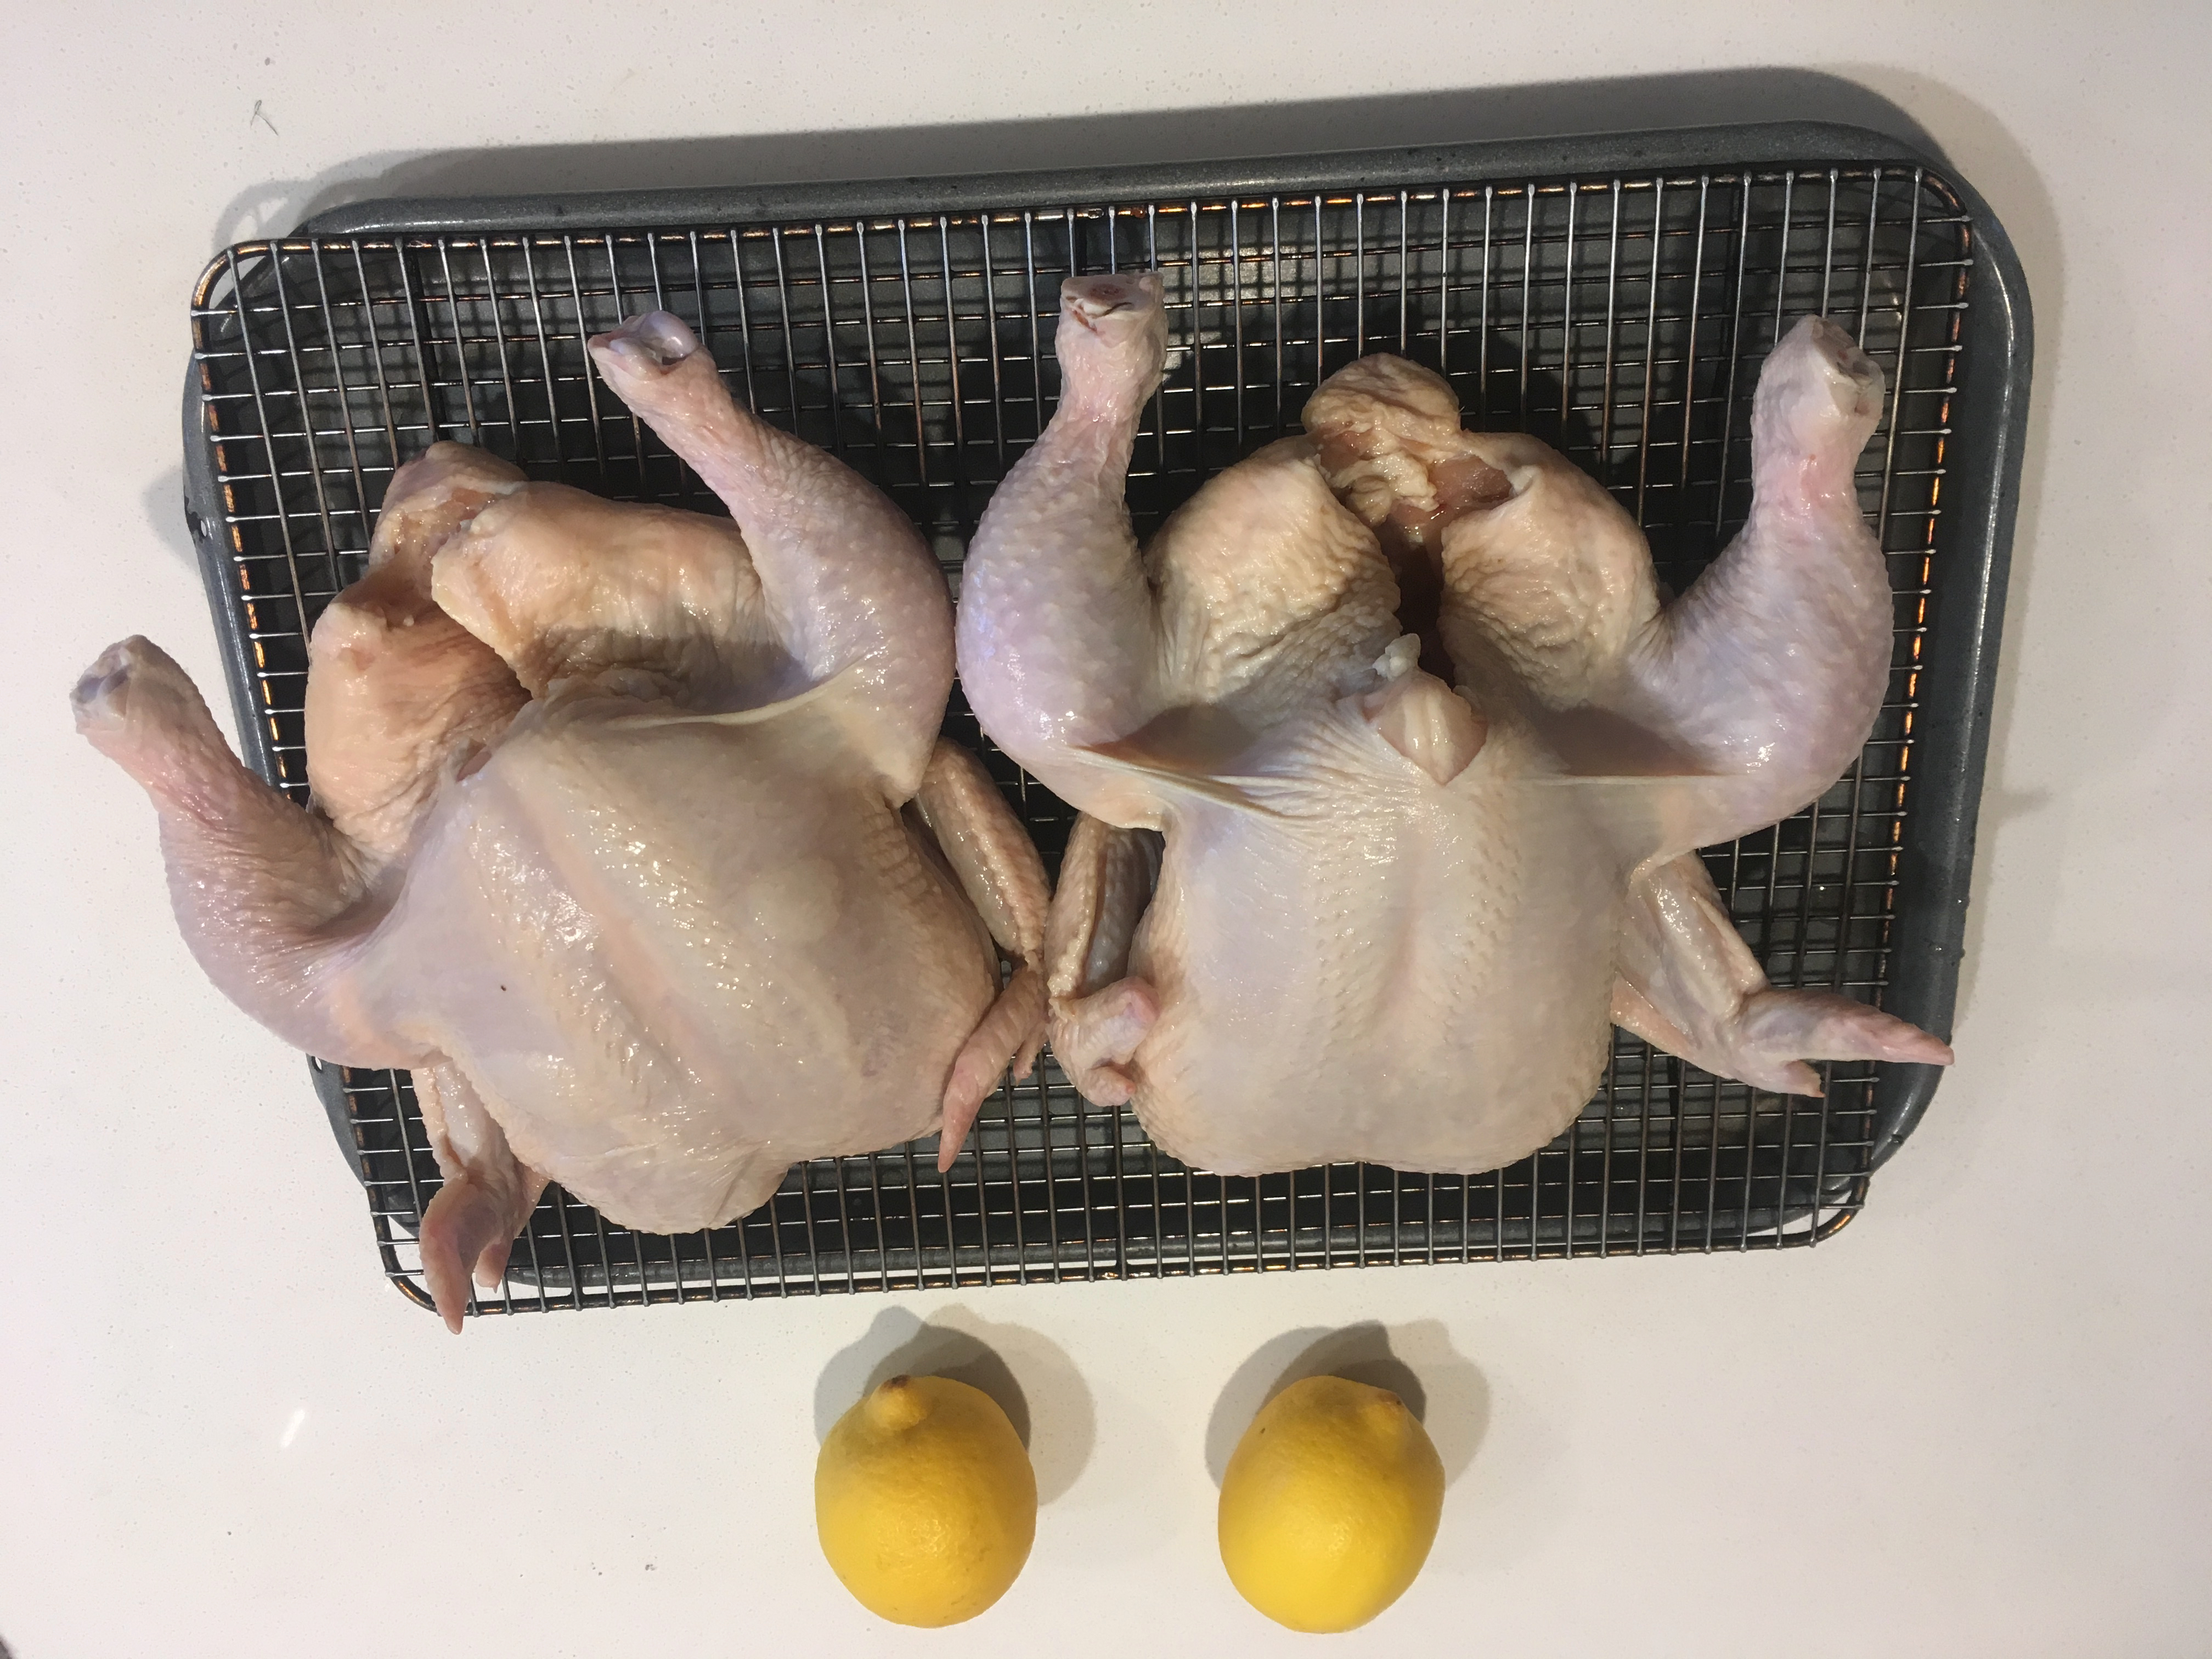
\includegraphics[width=0.25\textwidth]{\imageDir/\fileName/IMG_3197.jpg} &
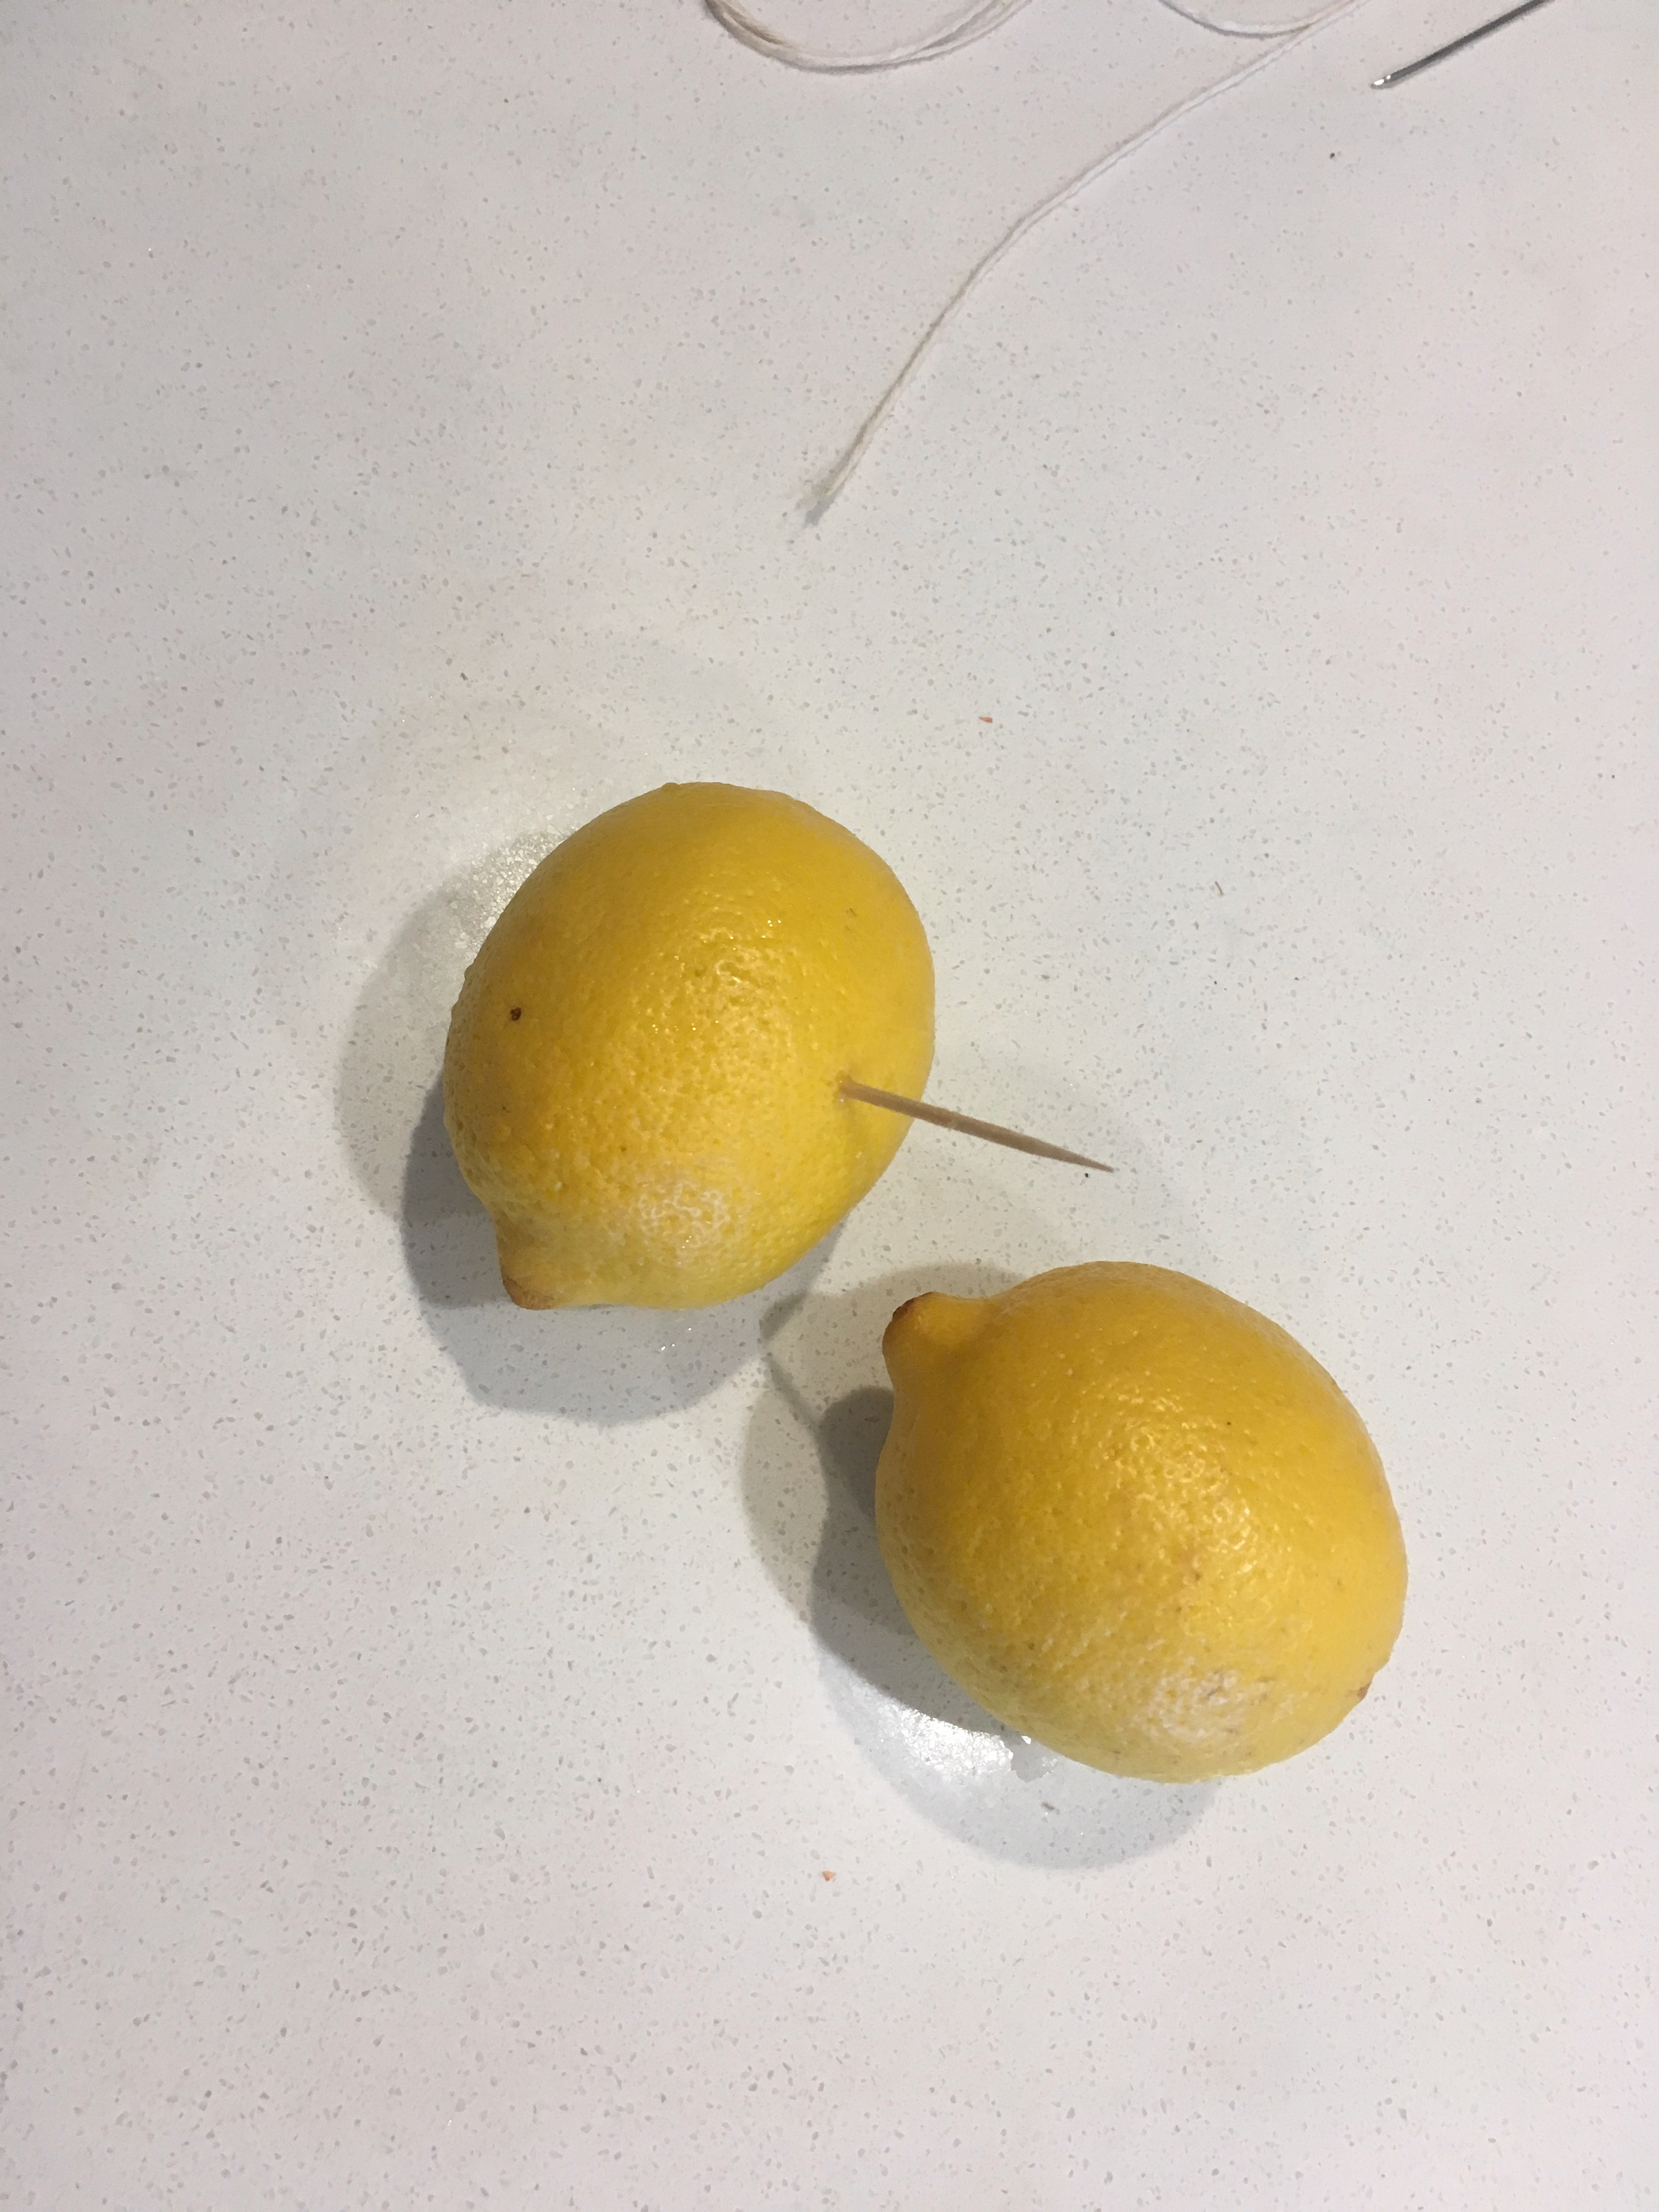
\includegraphics[width=0.25\textwidth]{\imageDir/\fileName/IMG_3212.jpg} &
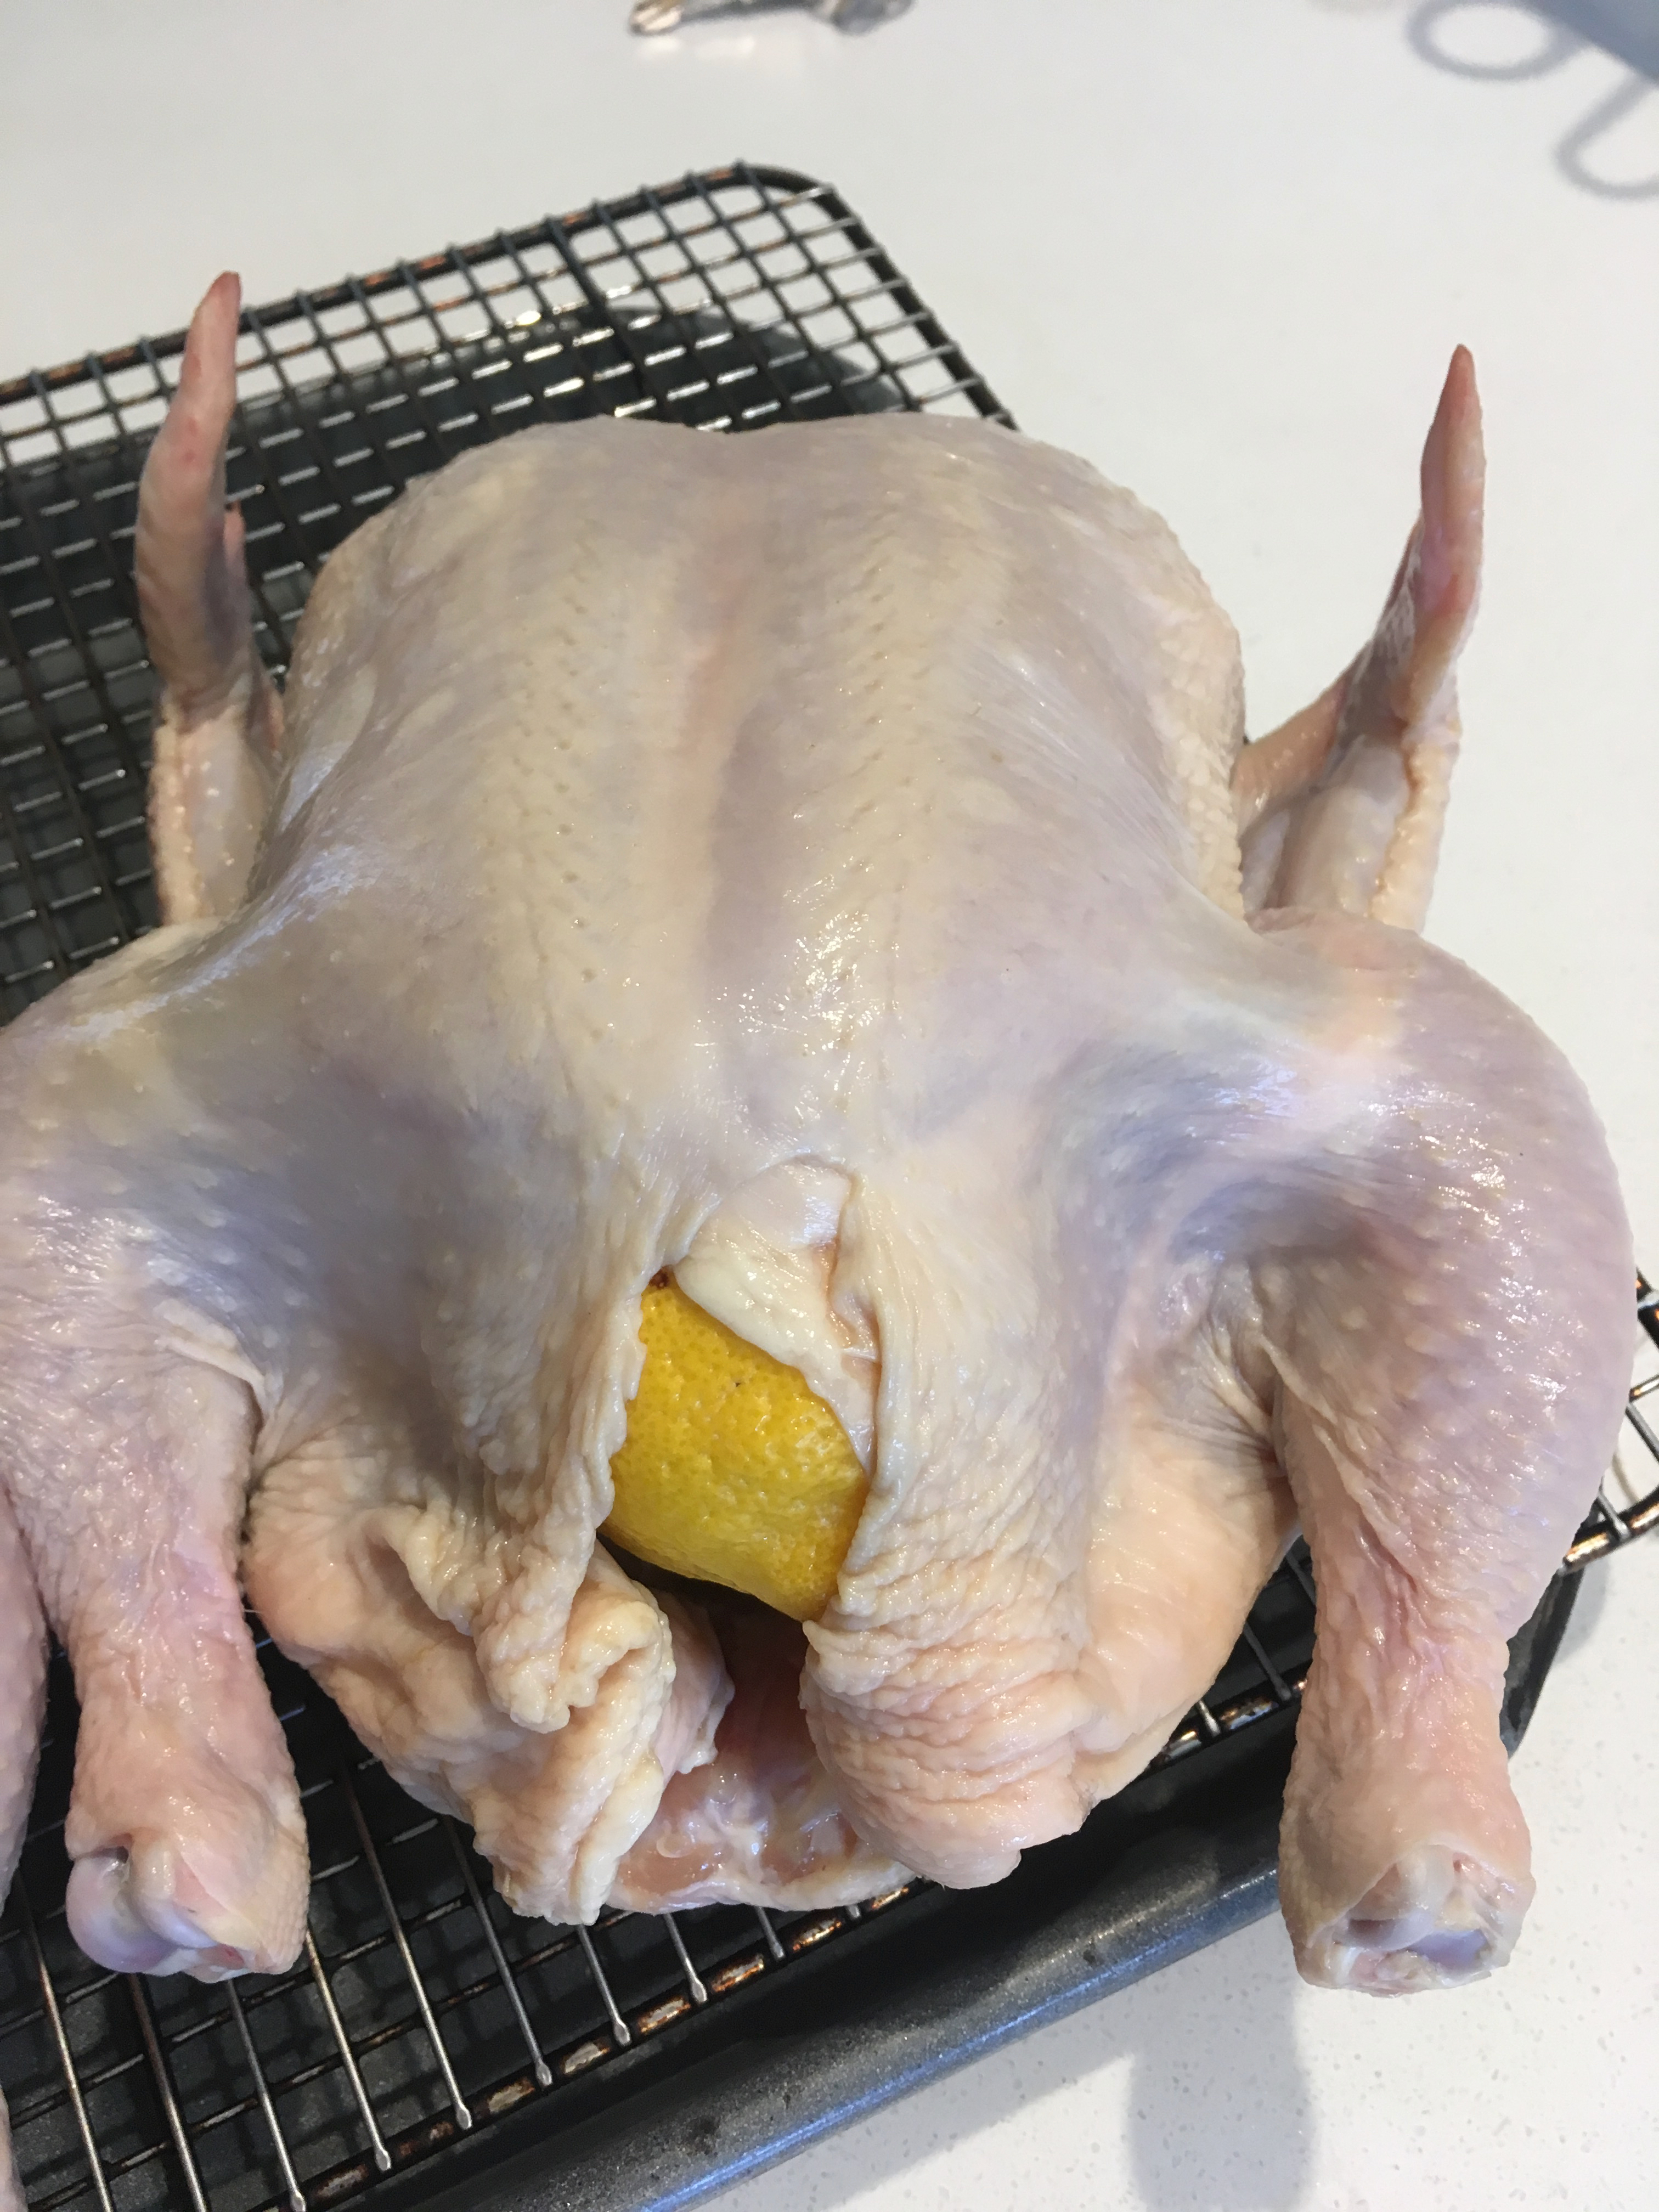
\includegraphics[width=0.25\textwidth]{\imageDir/\fileName/IMG_3213.jpg} \\
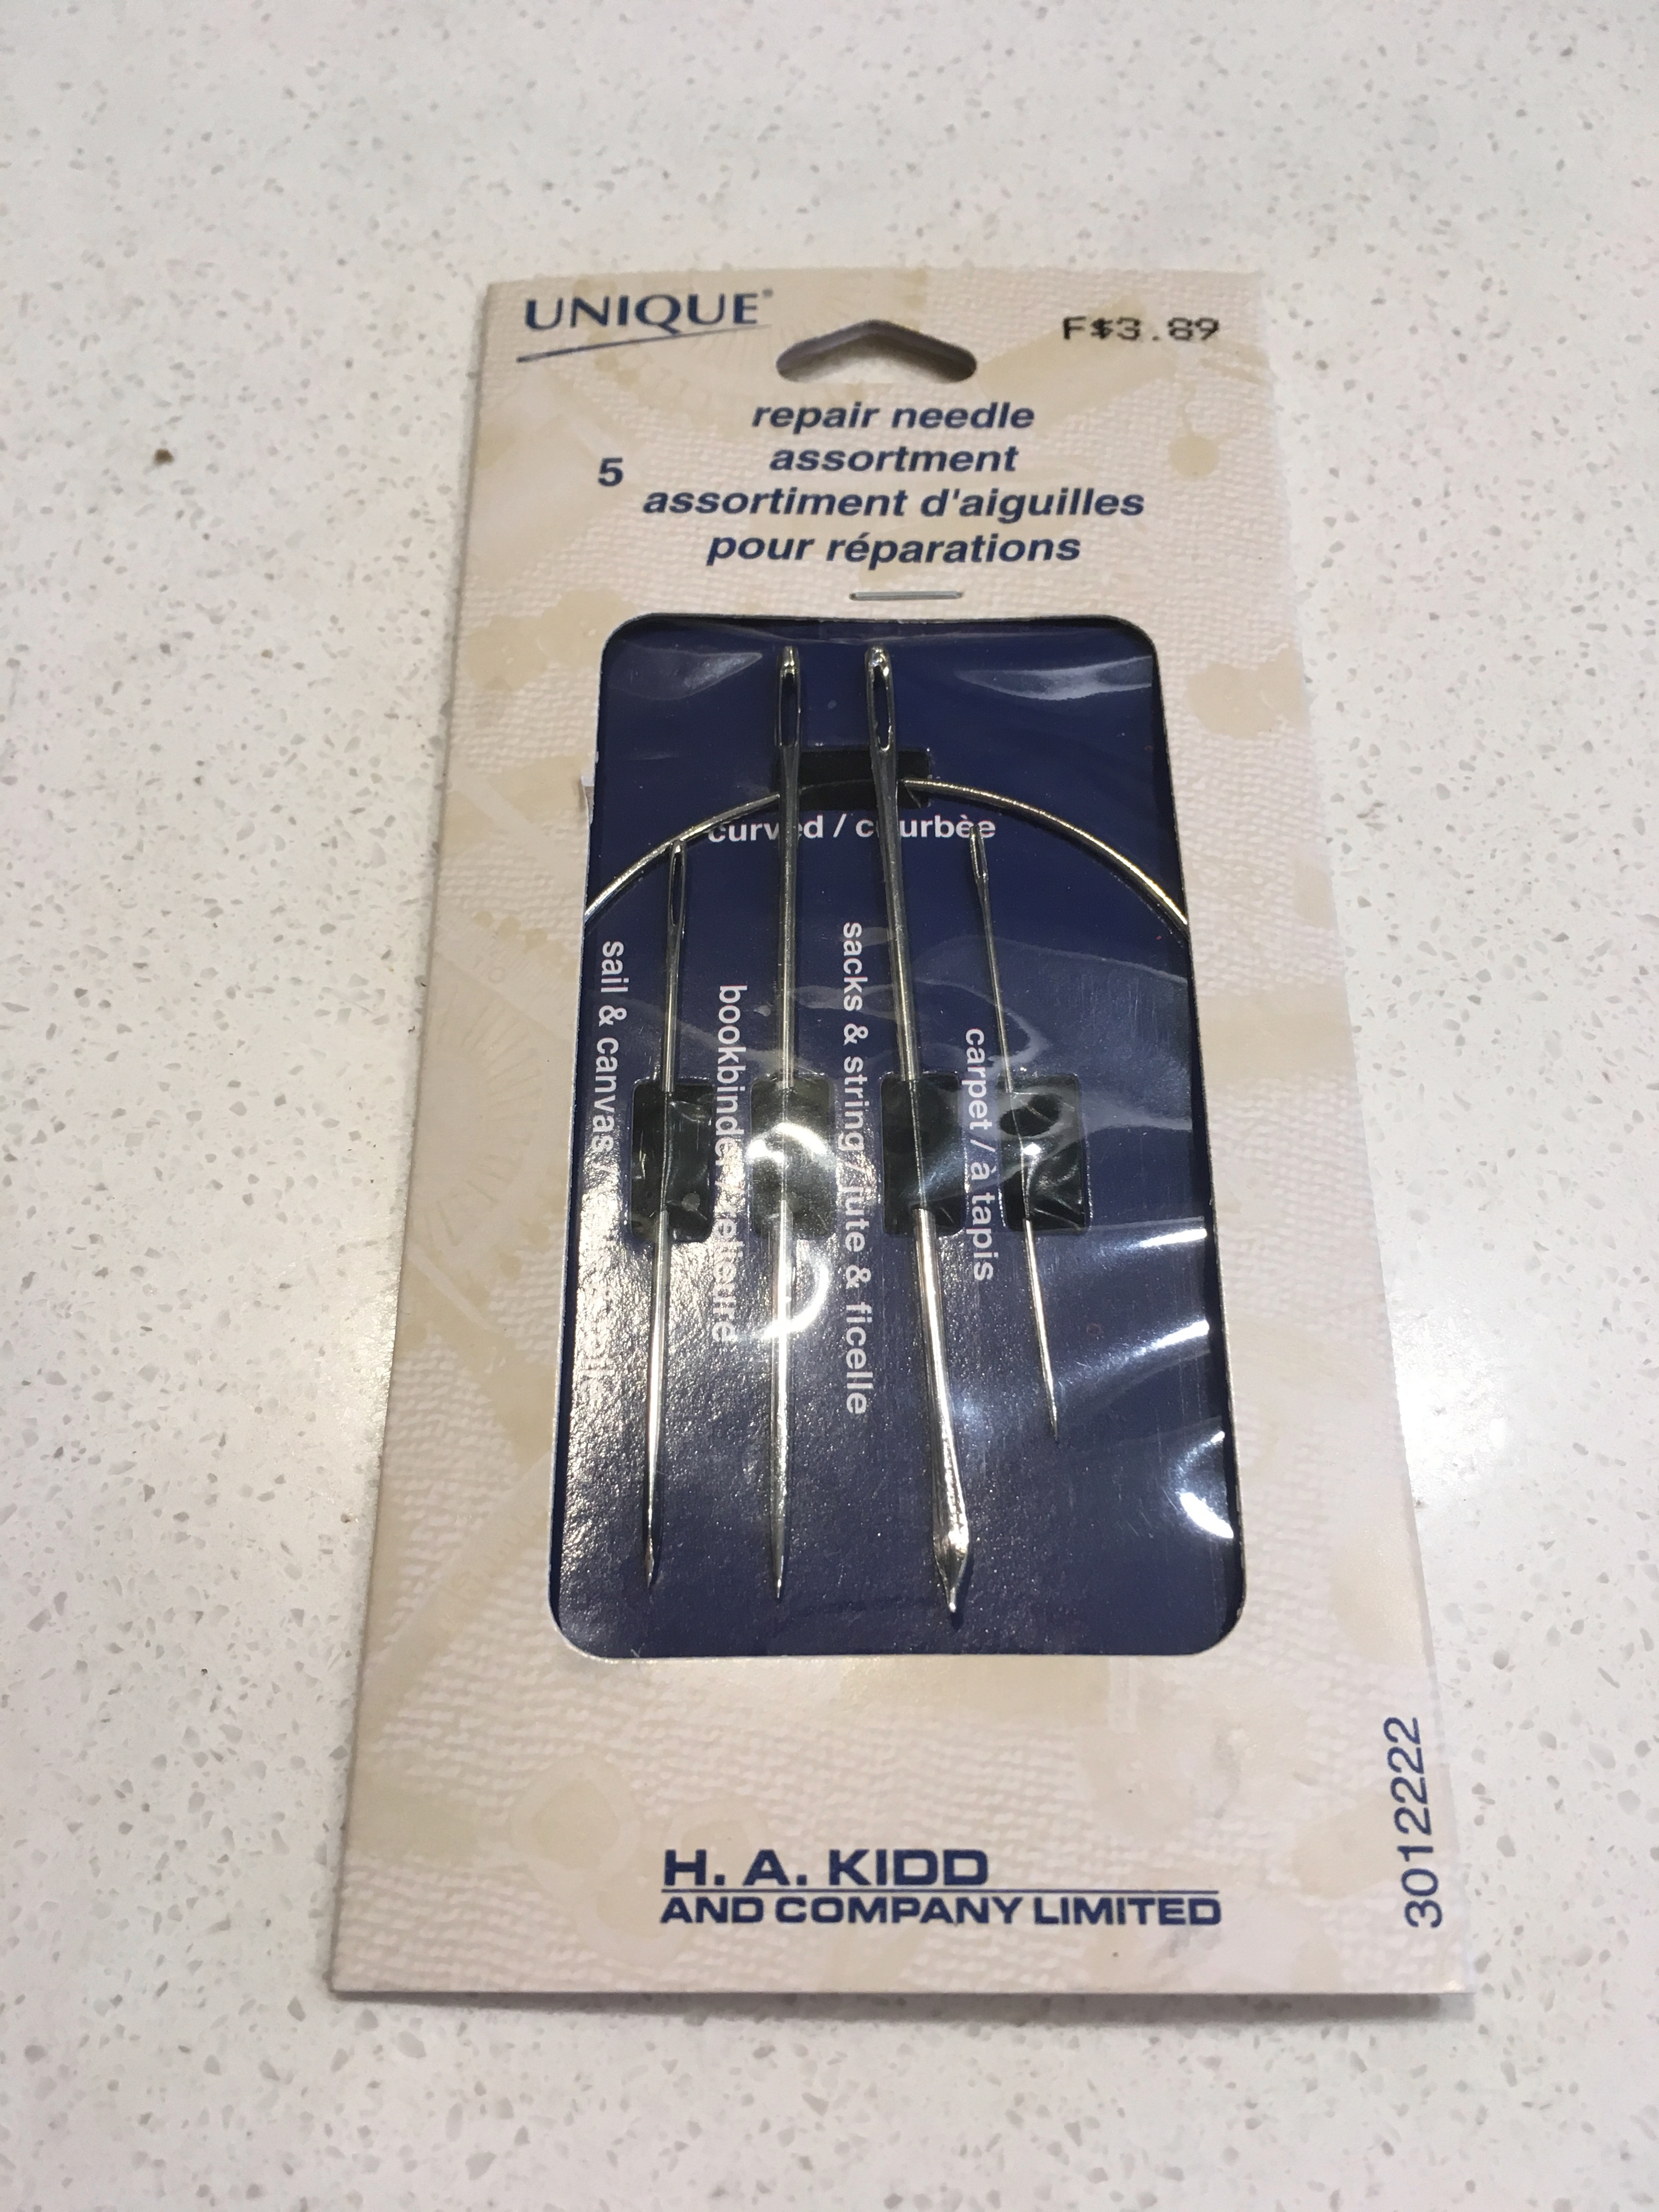
\includegraphics[width=0.25\textwidth]{\imageDir/\fileName/IMG_3206.jpg} &
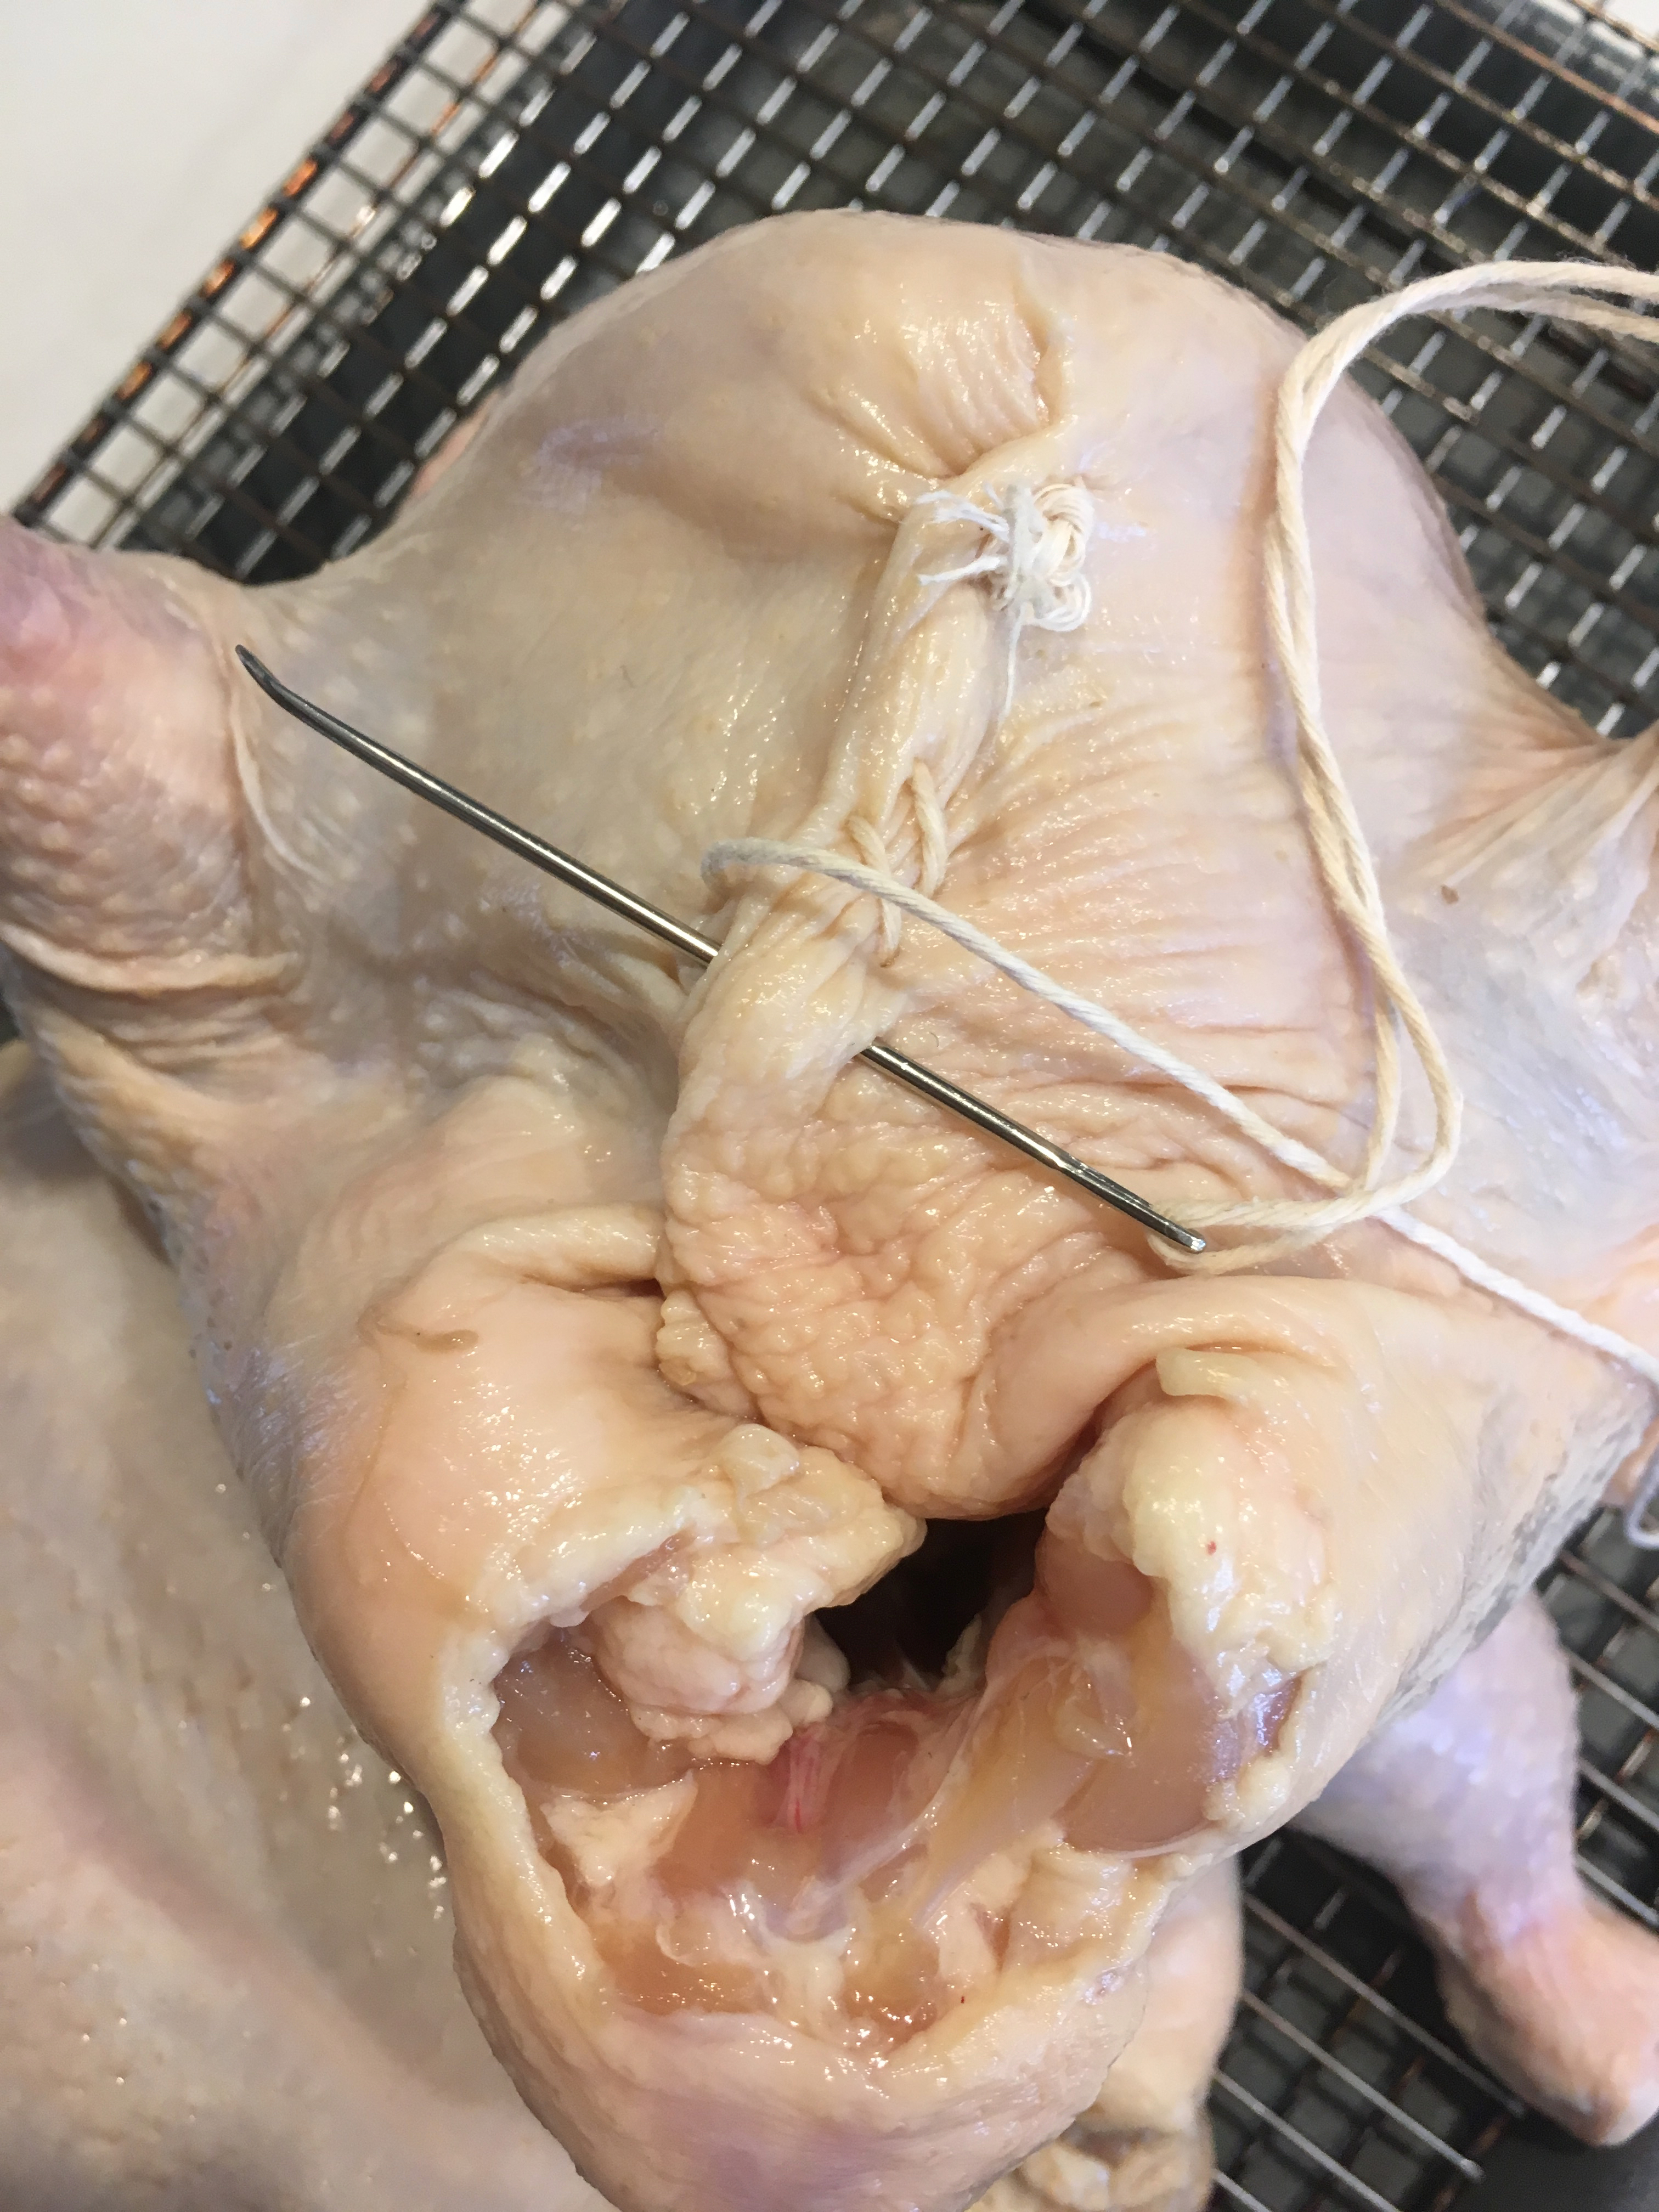
\includegraphics[width=0.25\textwidth]{\imageDir/\fileName/IMG_3214.jpg} &
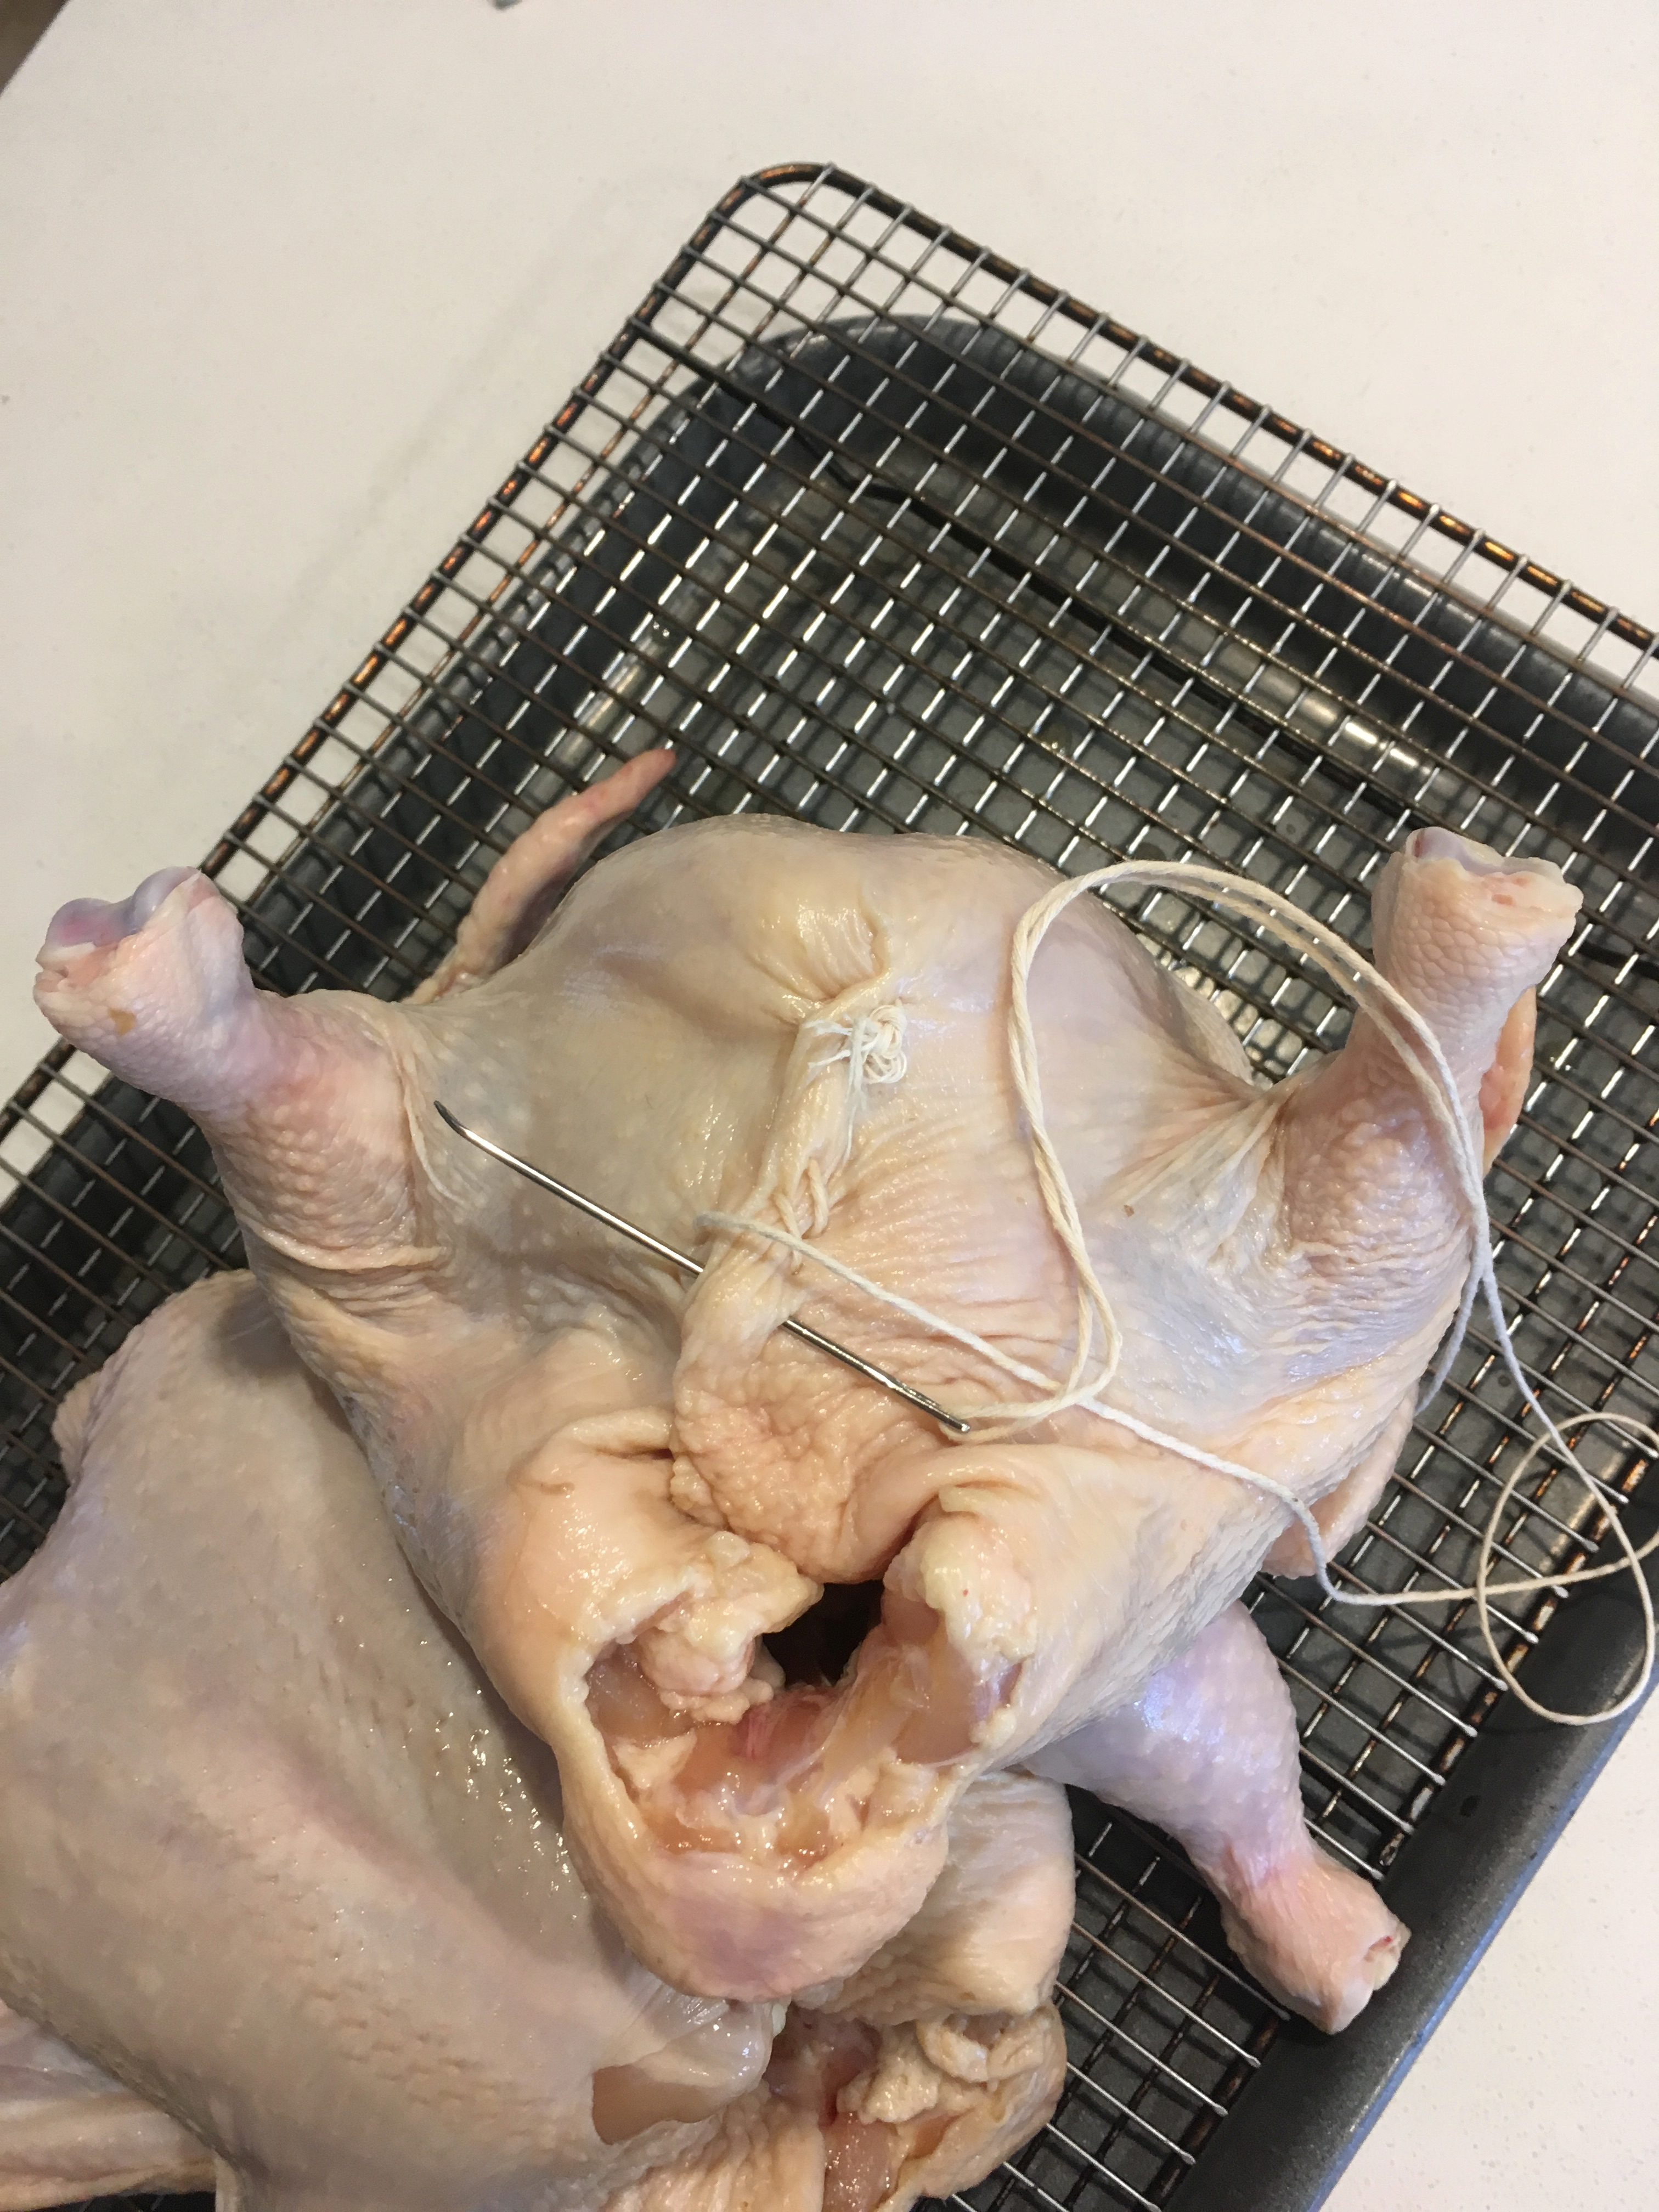
\includegraphics[width=0.25\textwidth]{\imageDir/\fileName/IMG_3216.jpg} \\
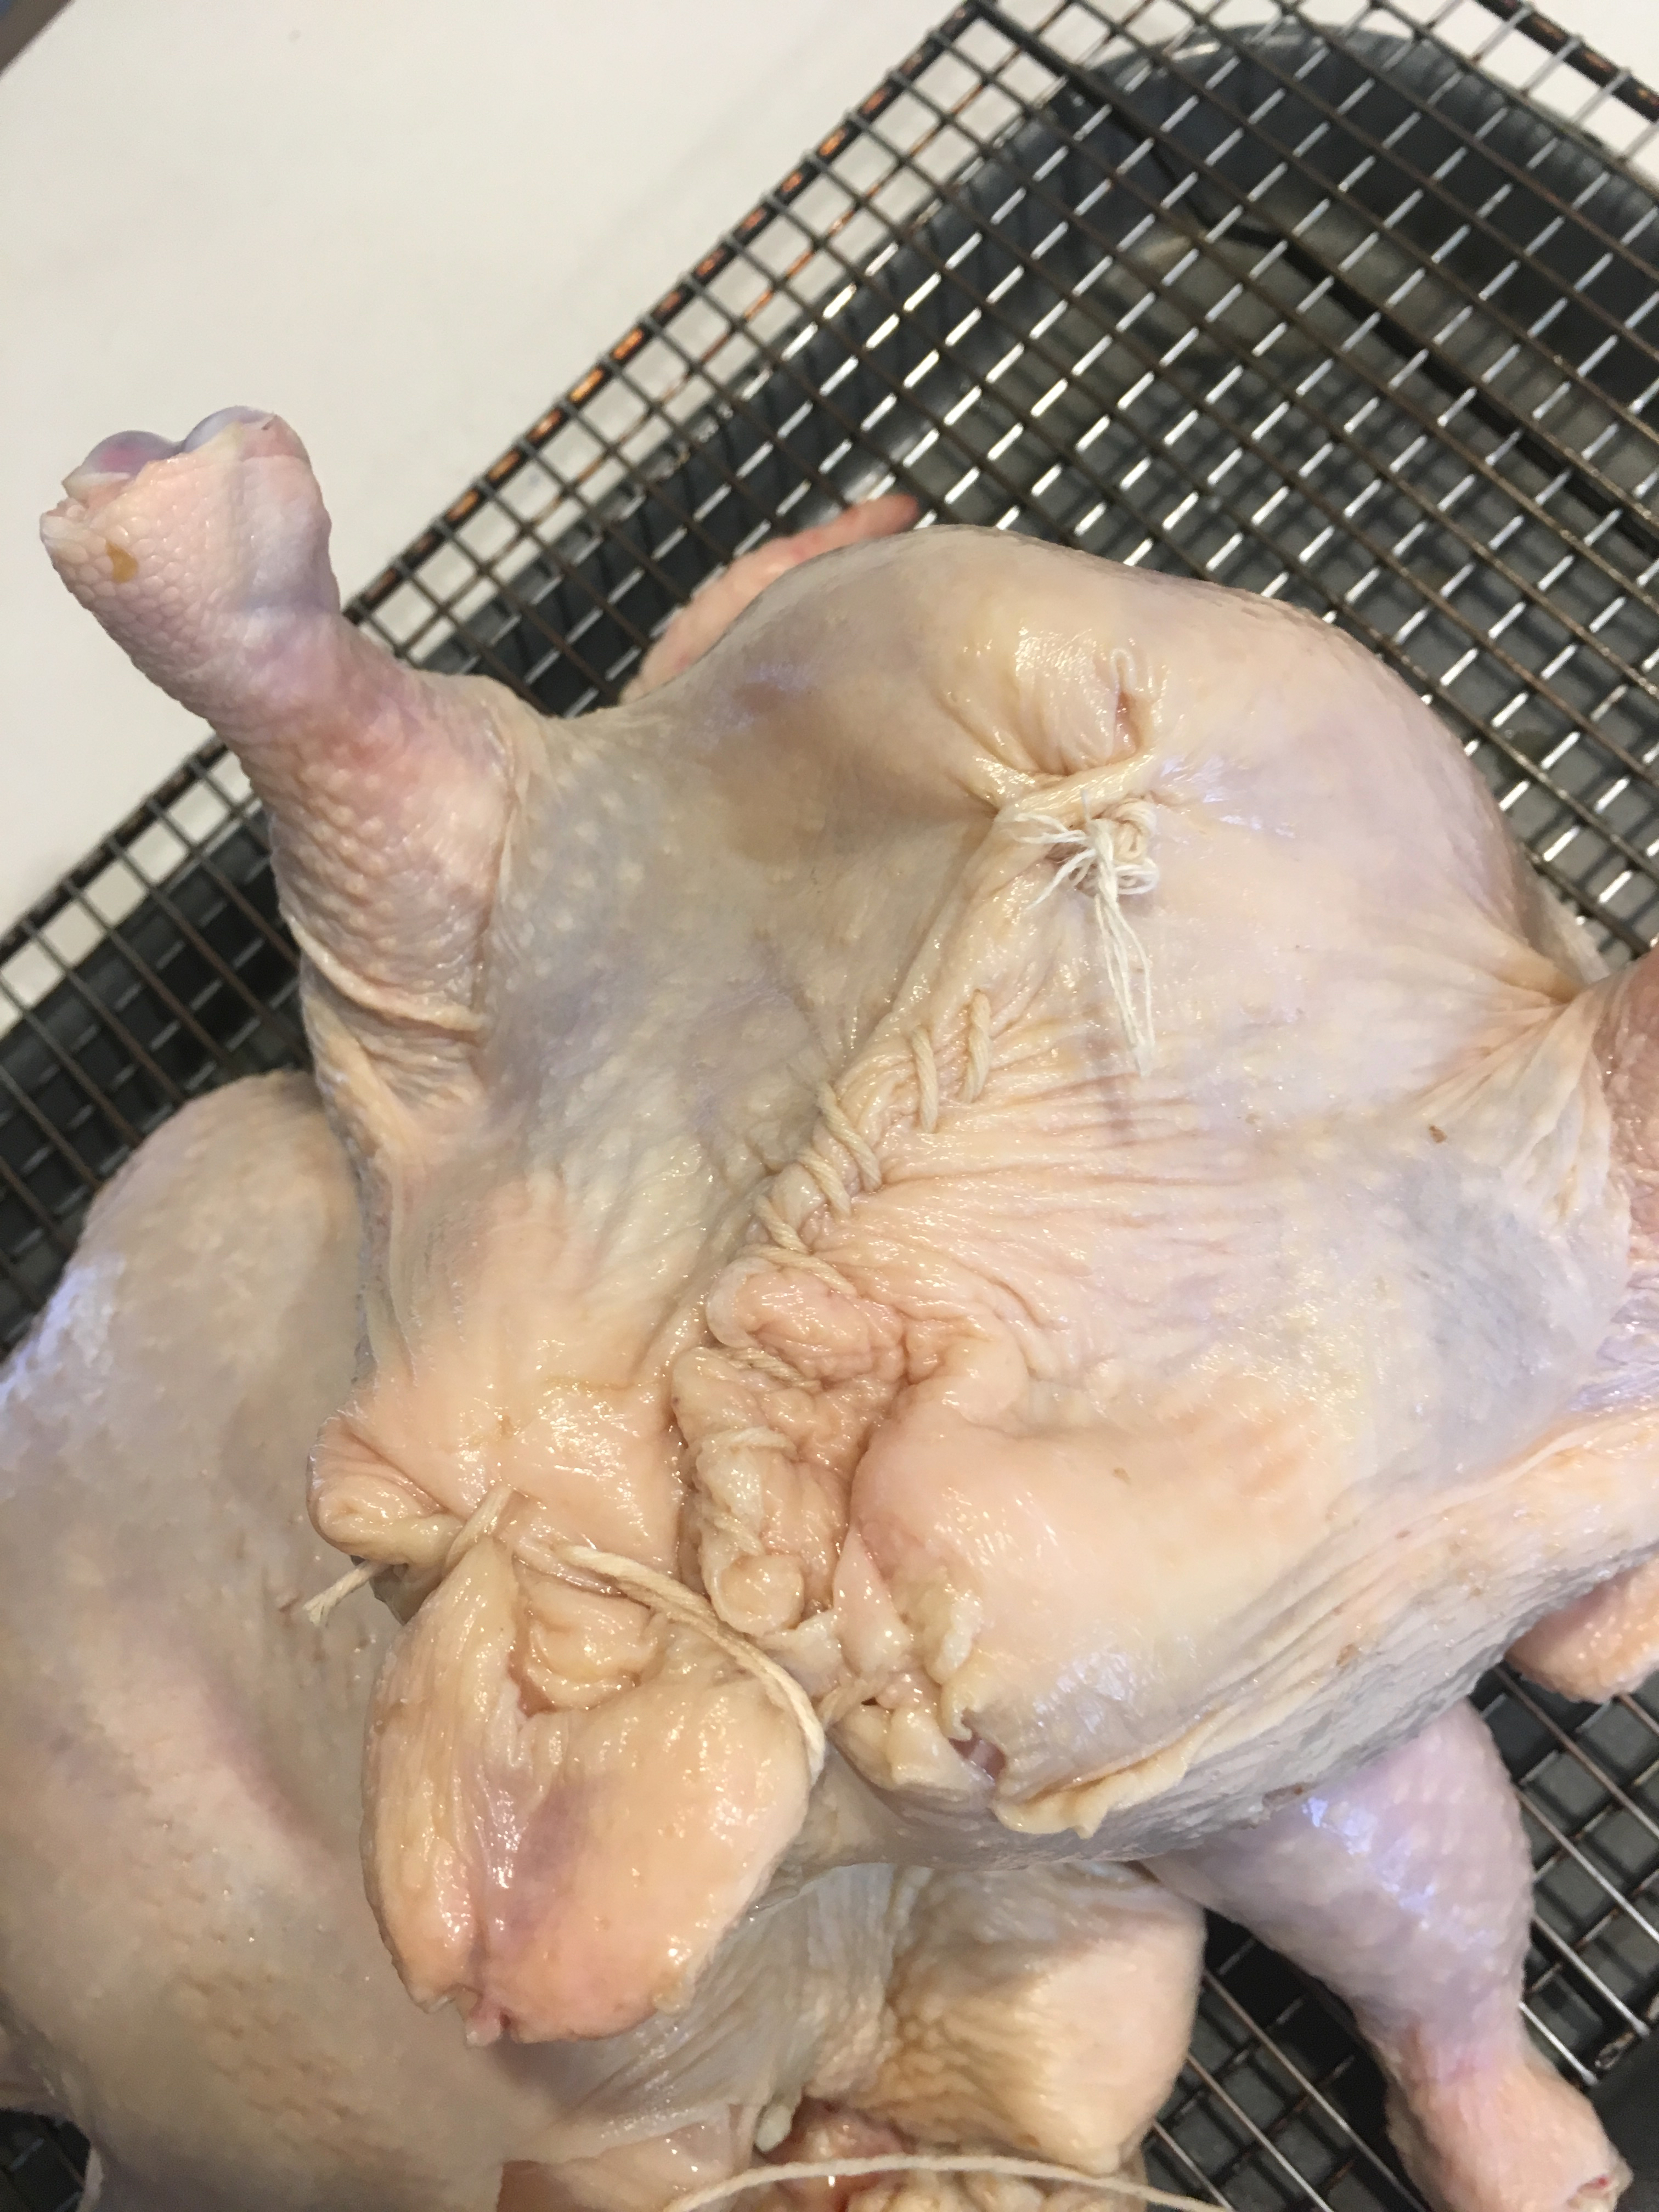
\includegraphics[width=0.25\textwidth]{\imageDir/\fileName/IMG_3217.jpg} &
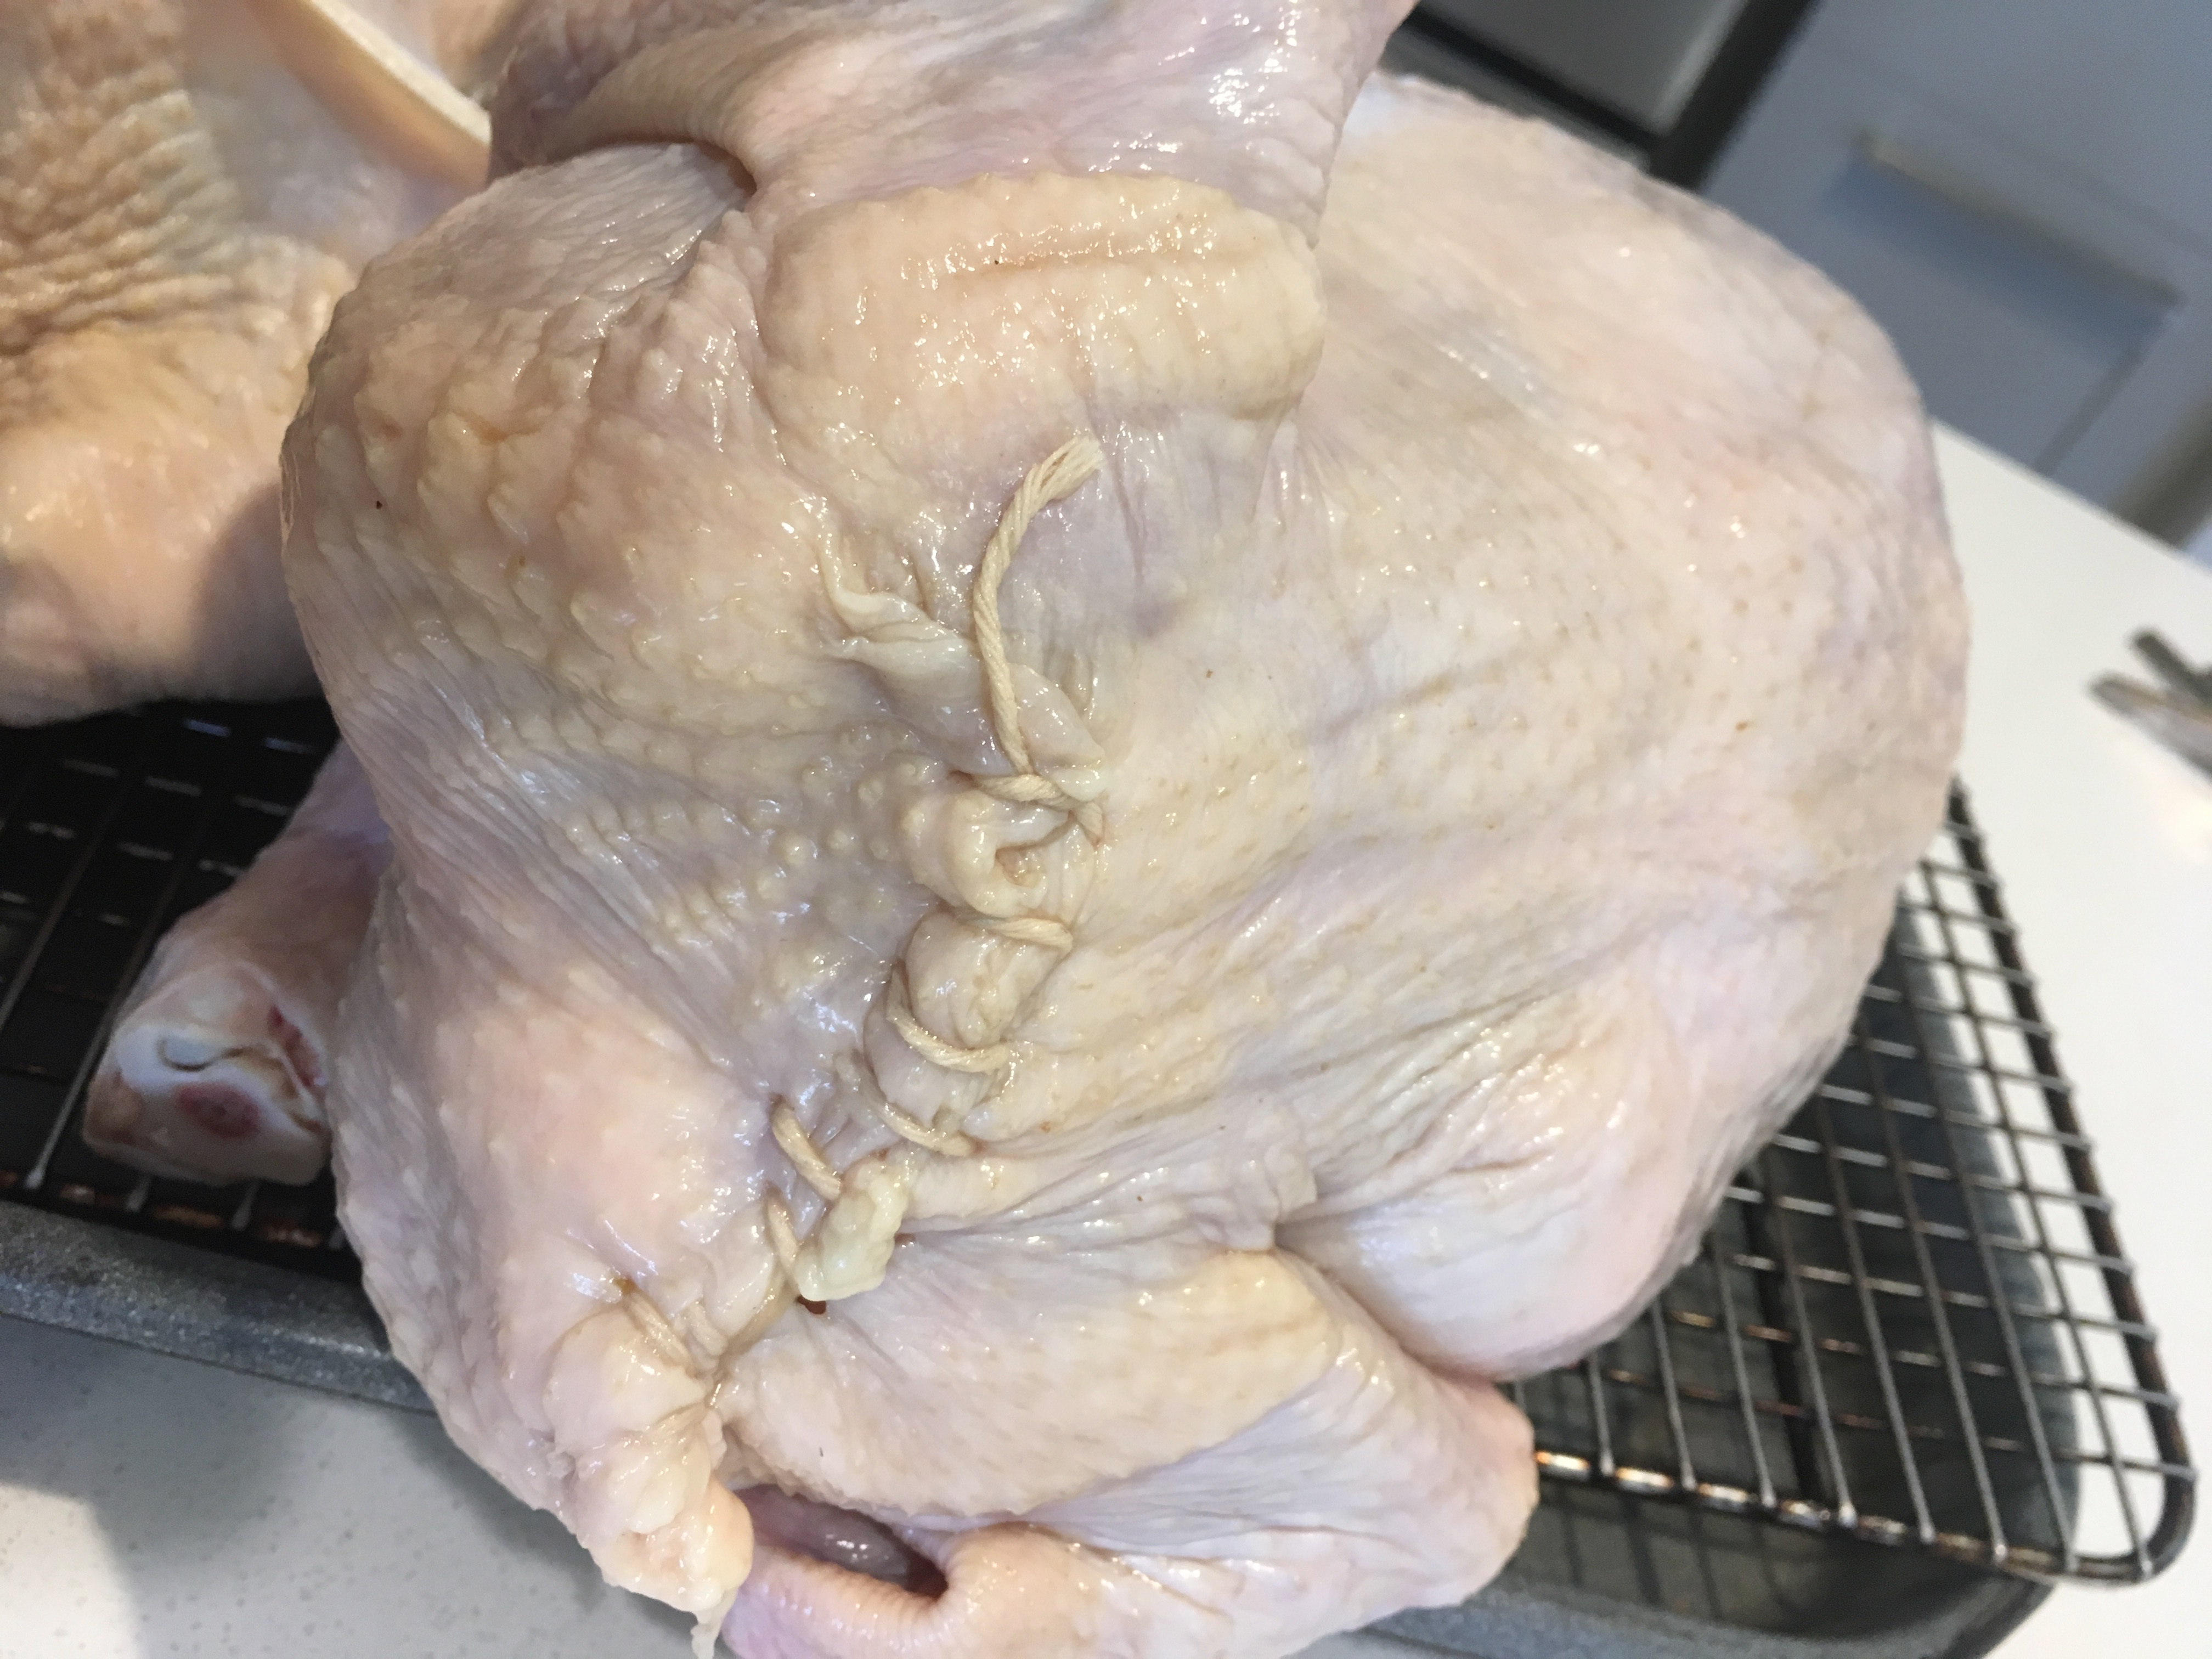
\includegraphics[width=0.25\textwidth]{\imageDir/\fileName/IMG_3218.jpg} &
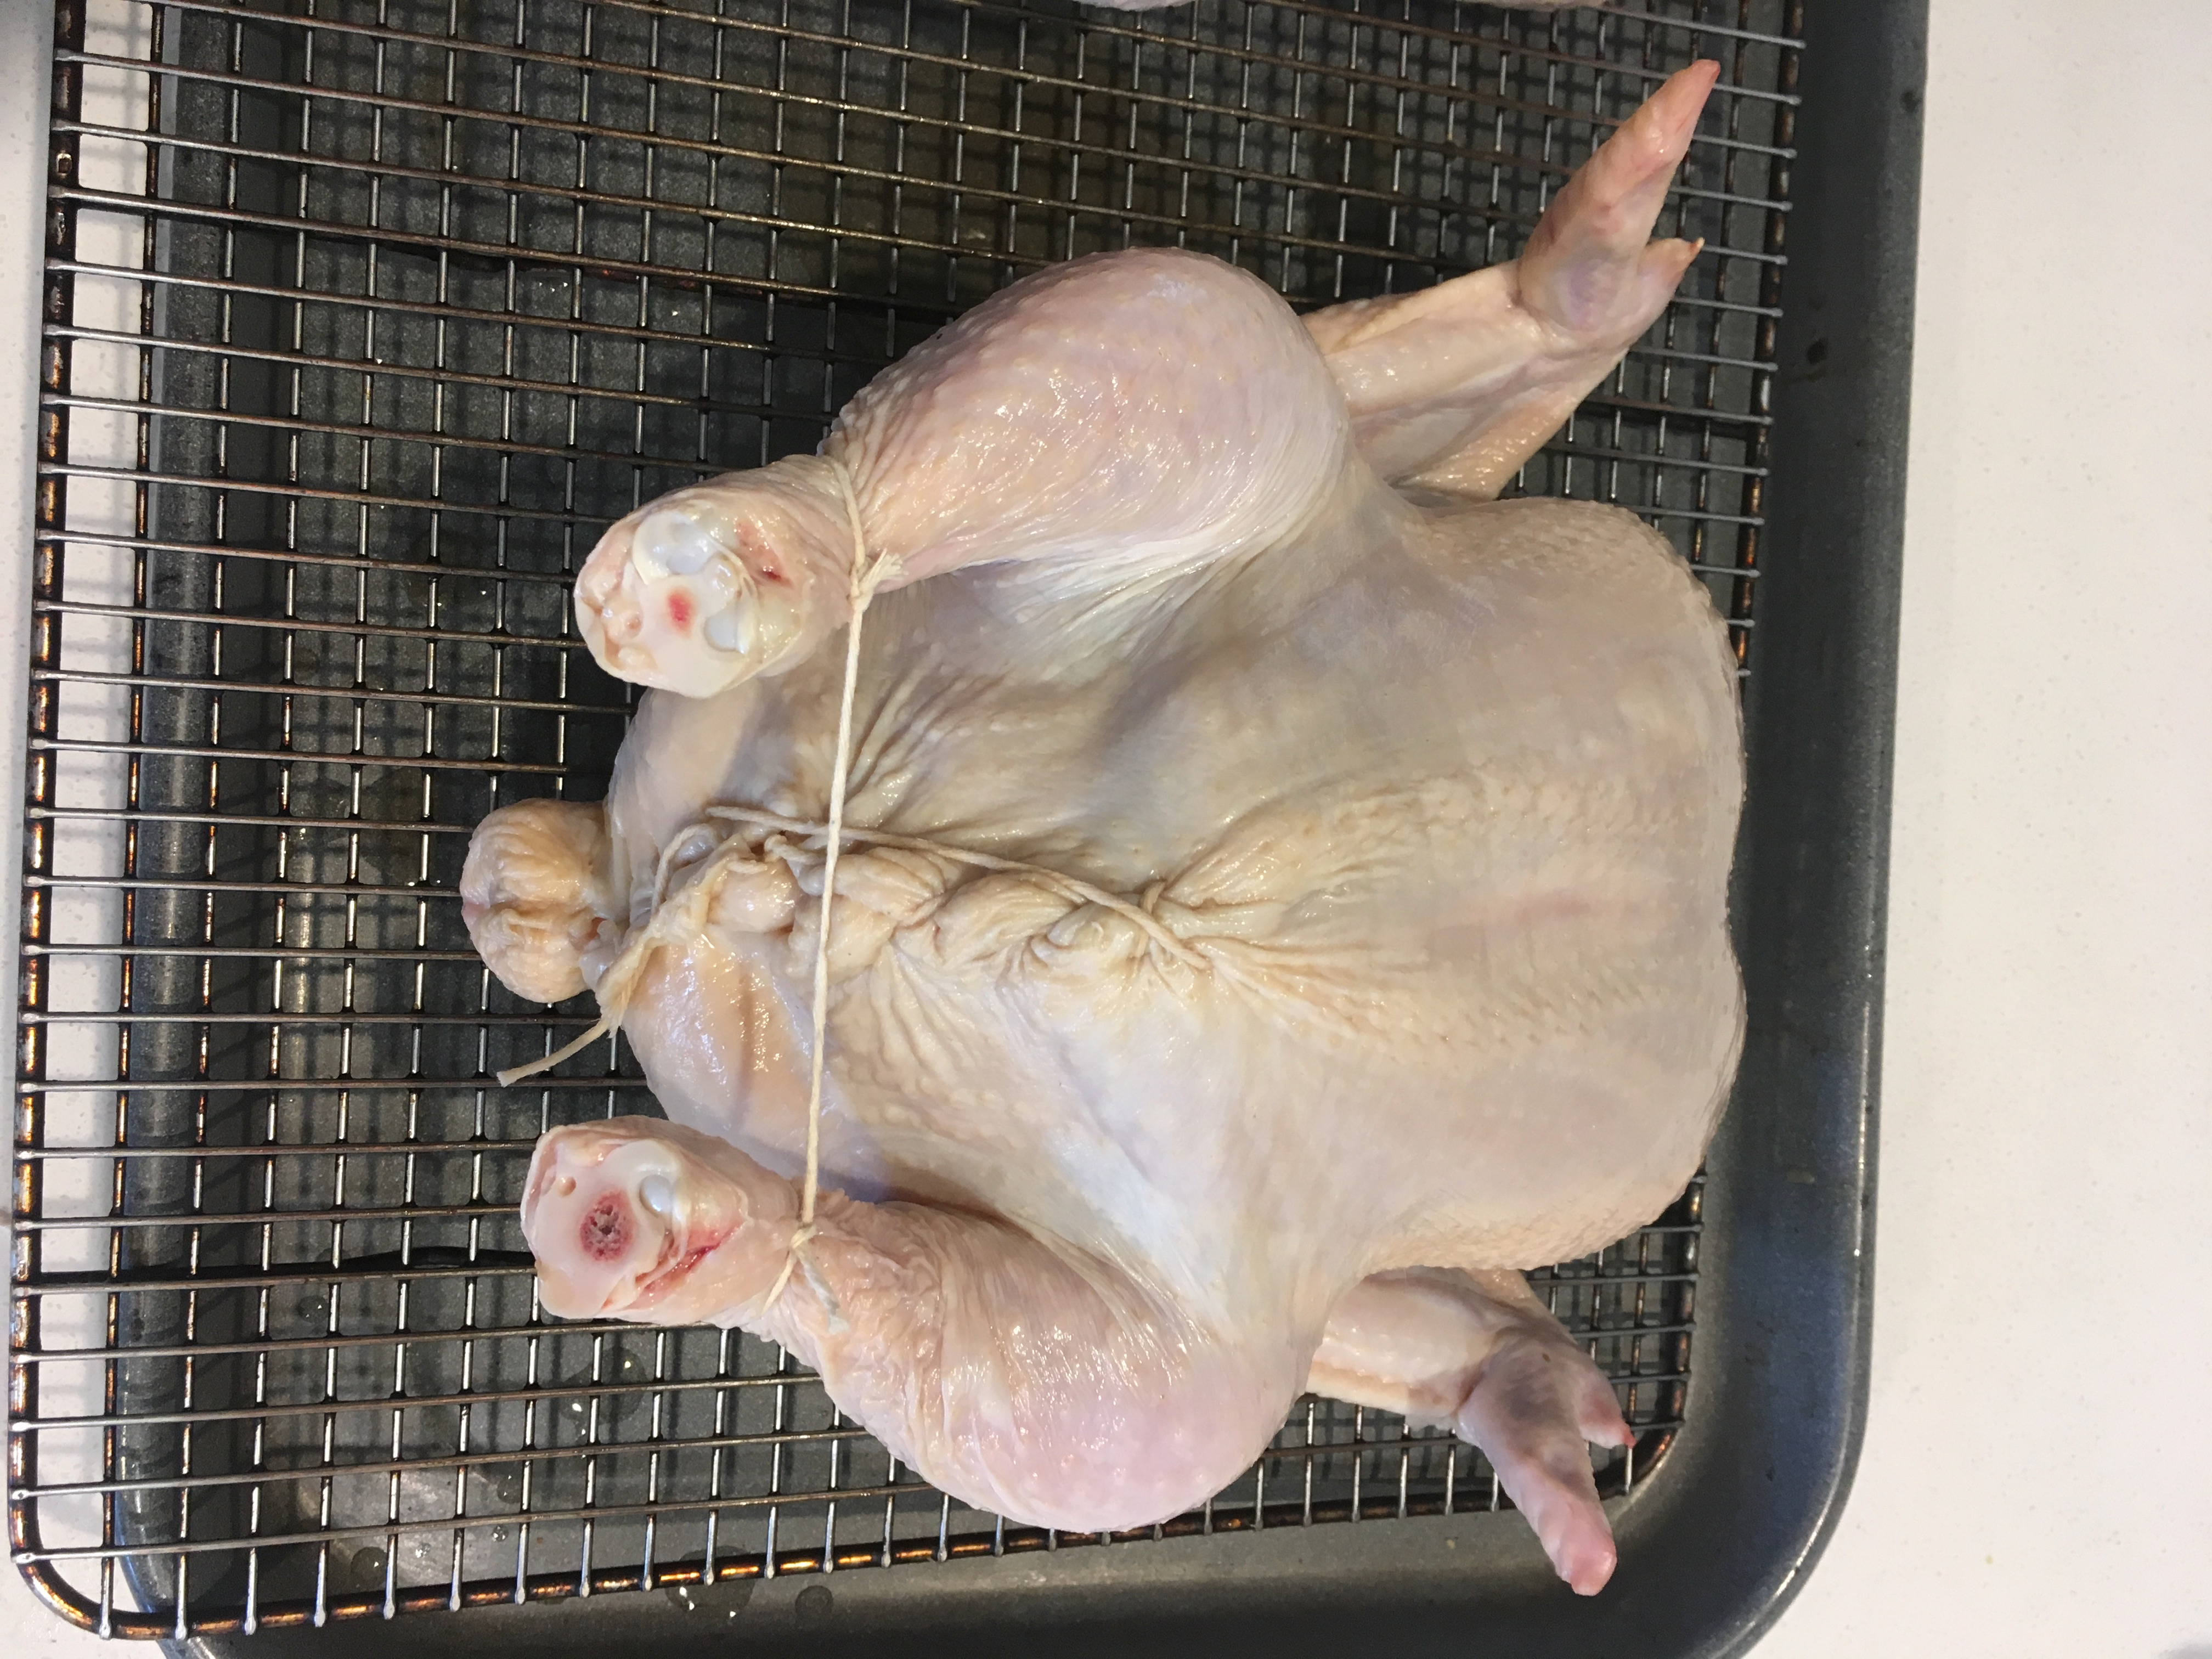
\includegraphics[width=0.25\textwidth]{\imageDir/\fileName/IMG_3219.jpg} \\
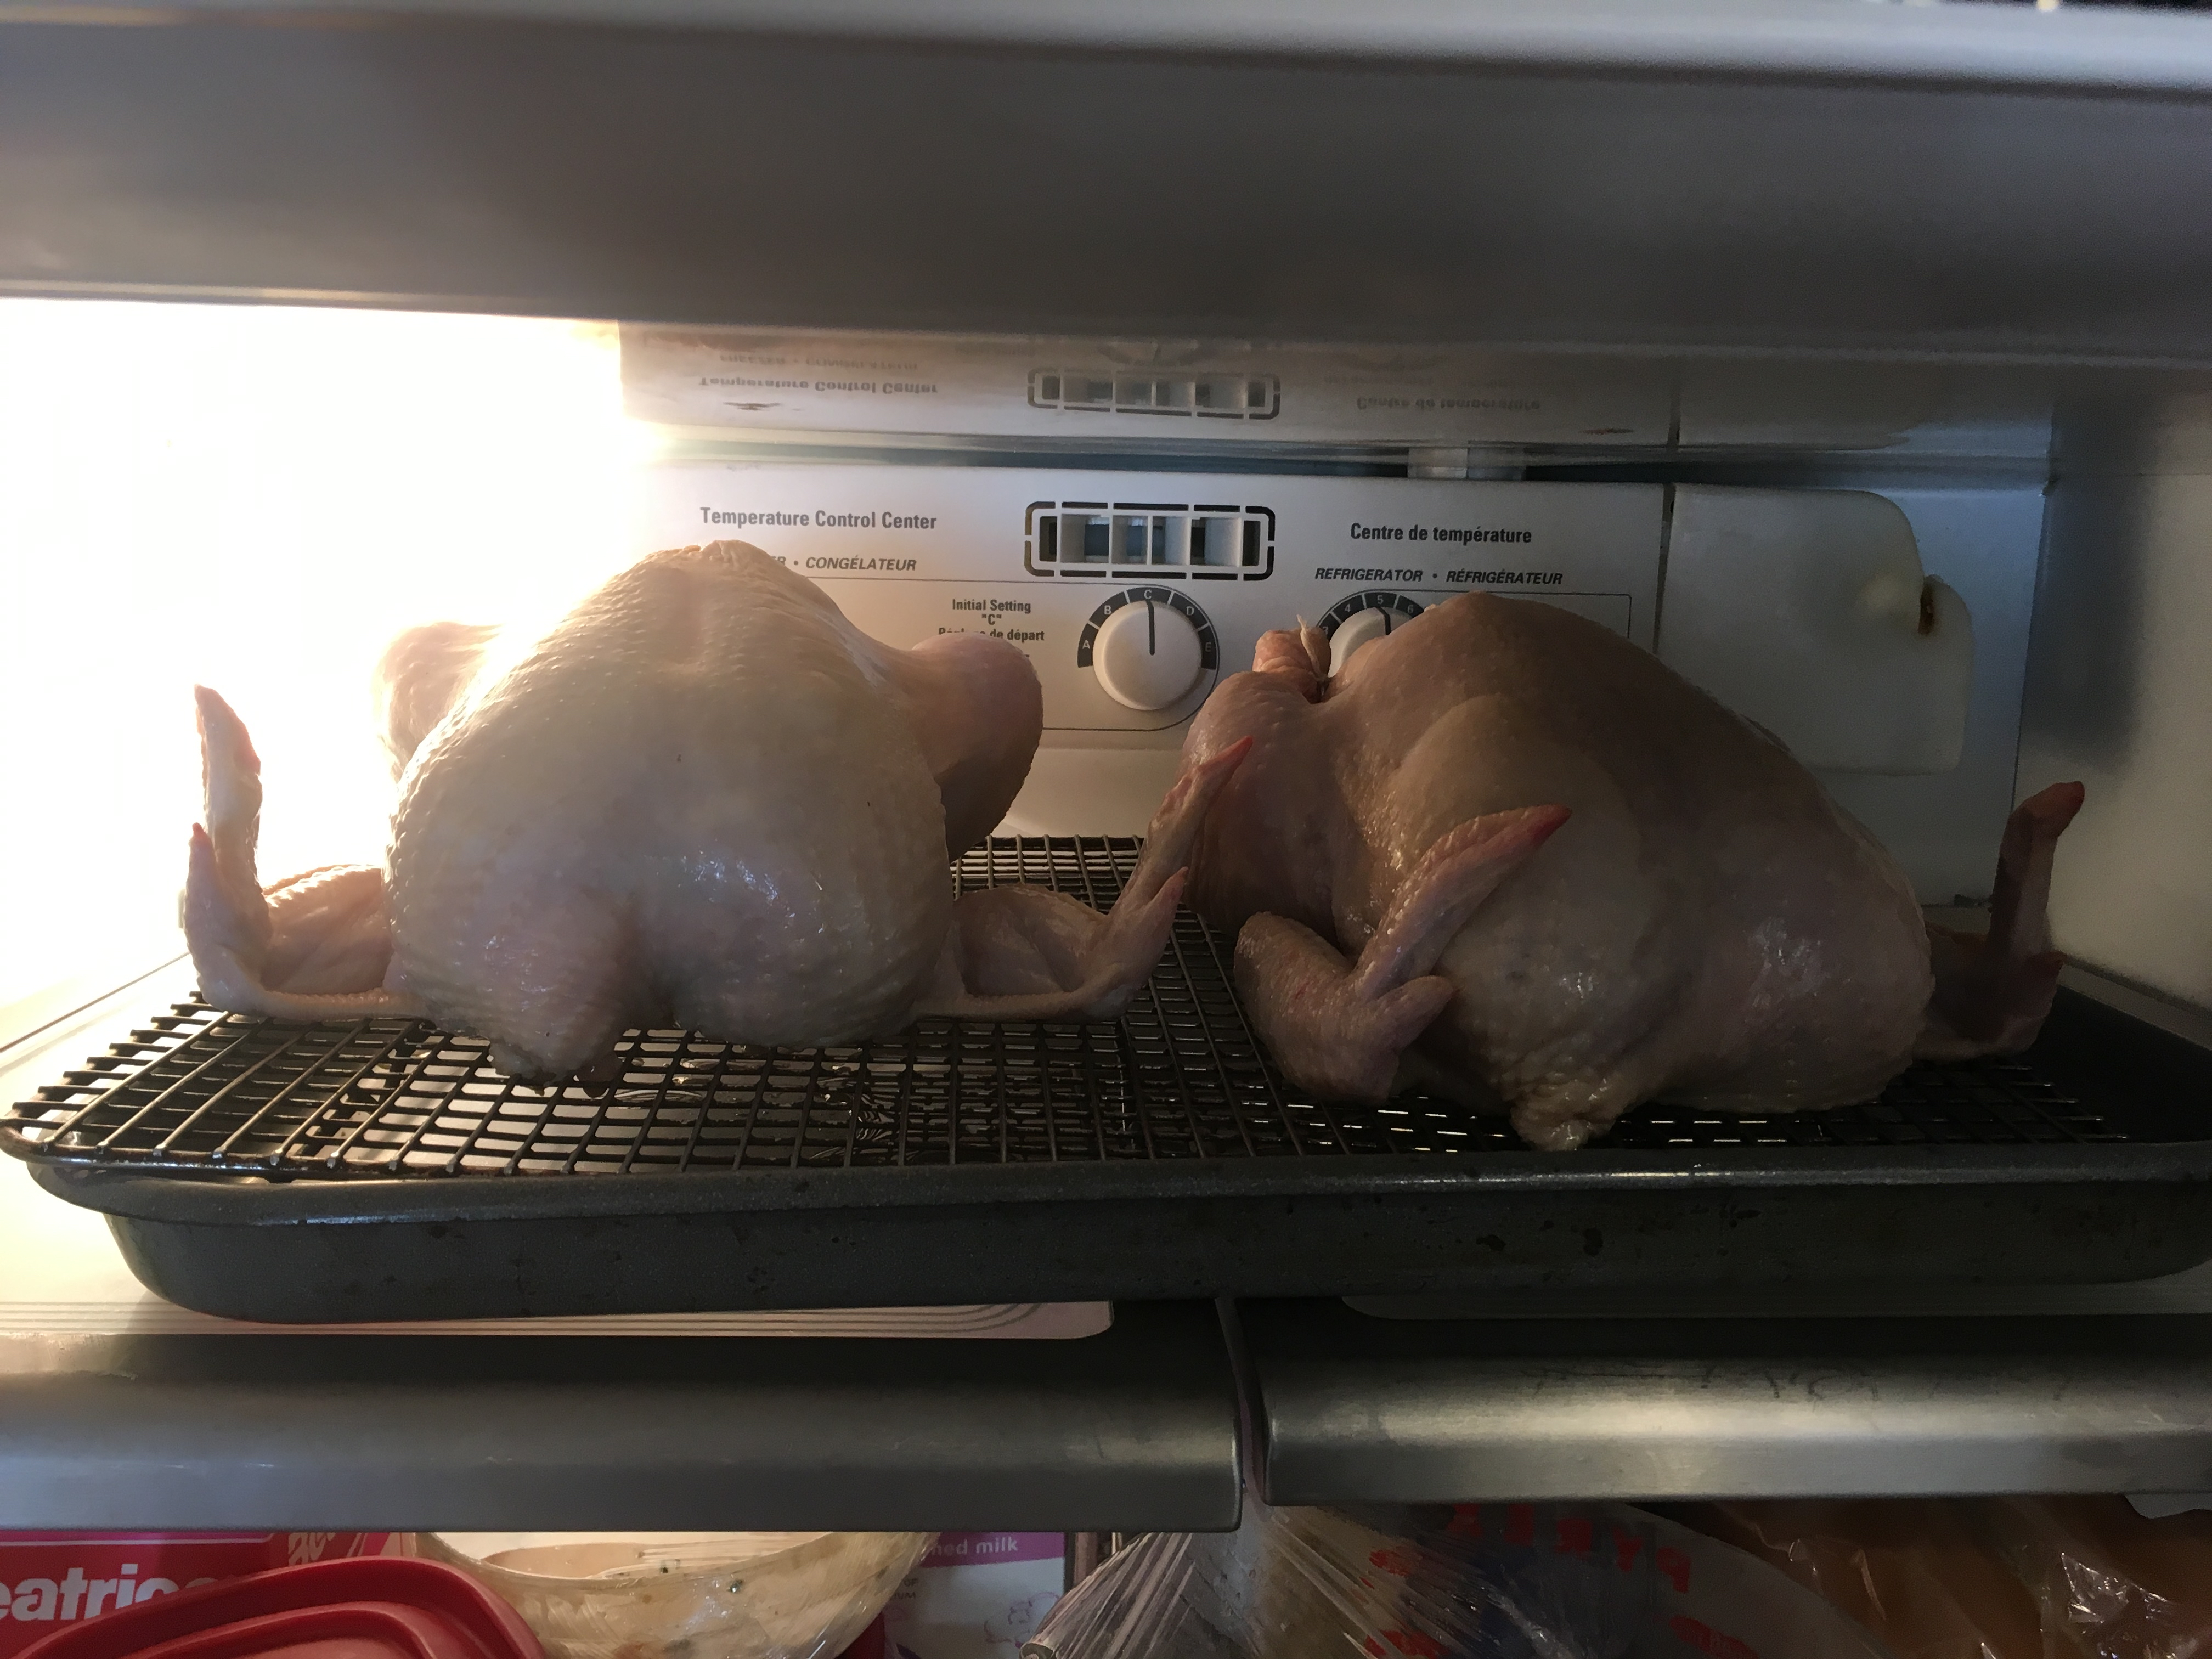
\includegraphics[width=0.25\textwidth]{\imageDir/\fileName/IMG_3220.jpg} &
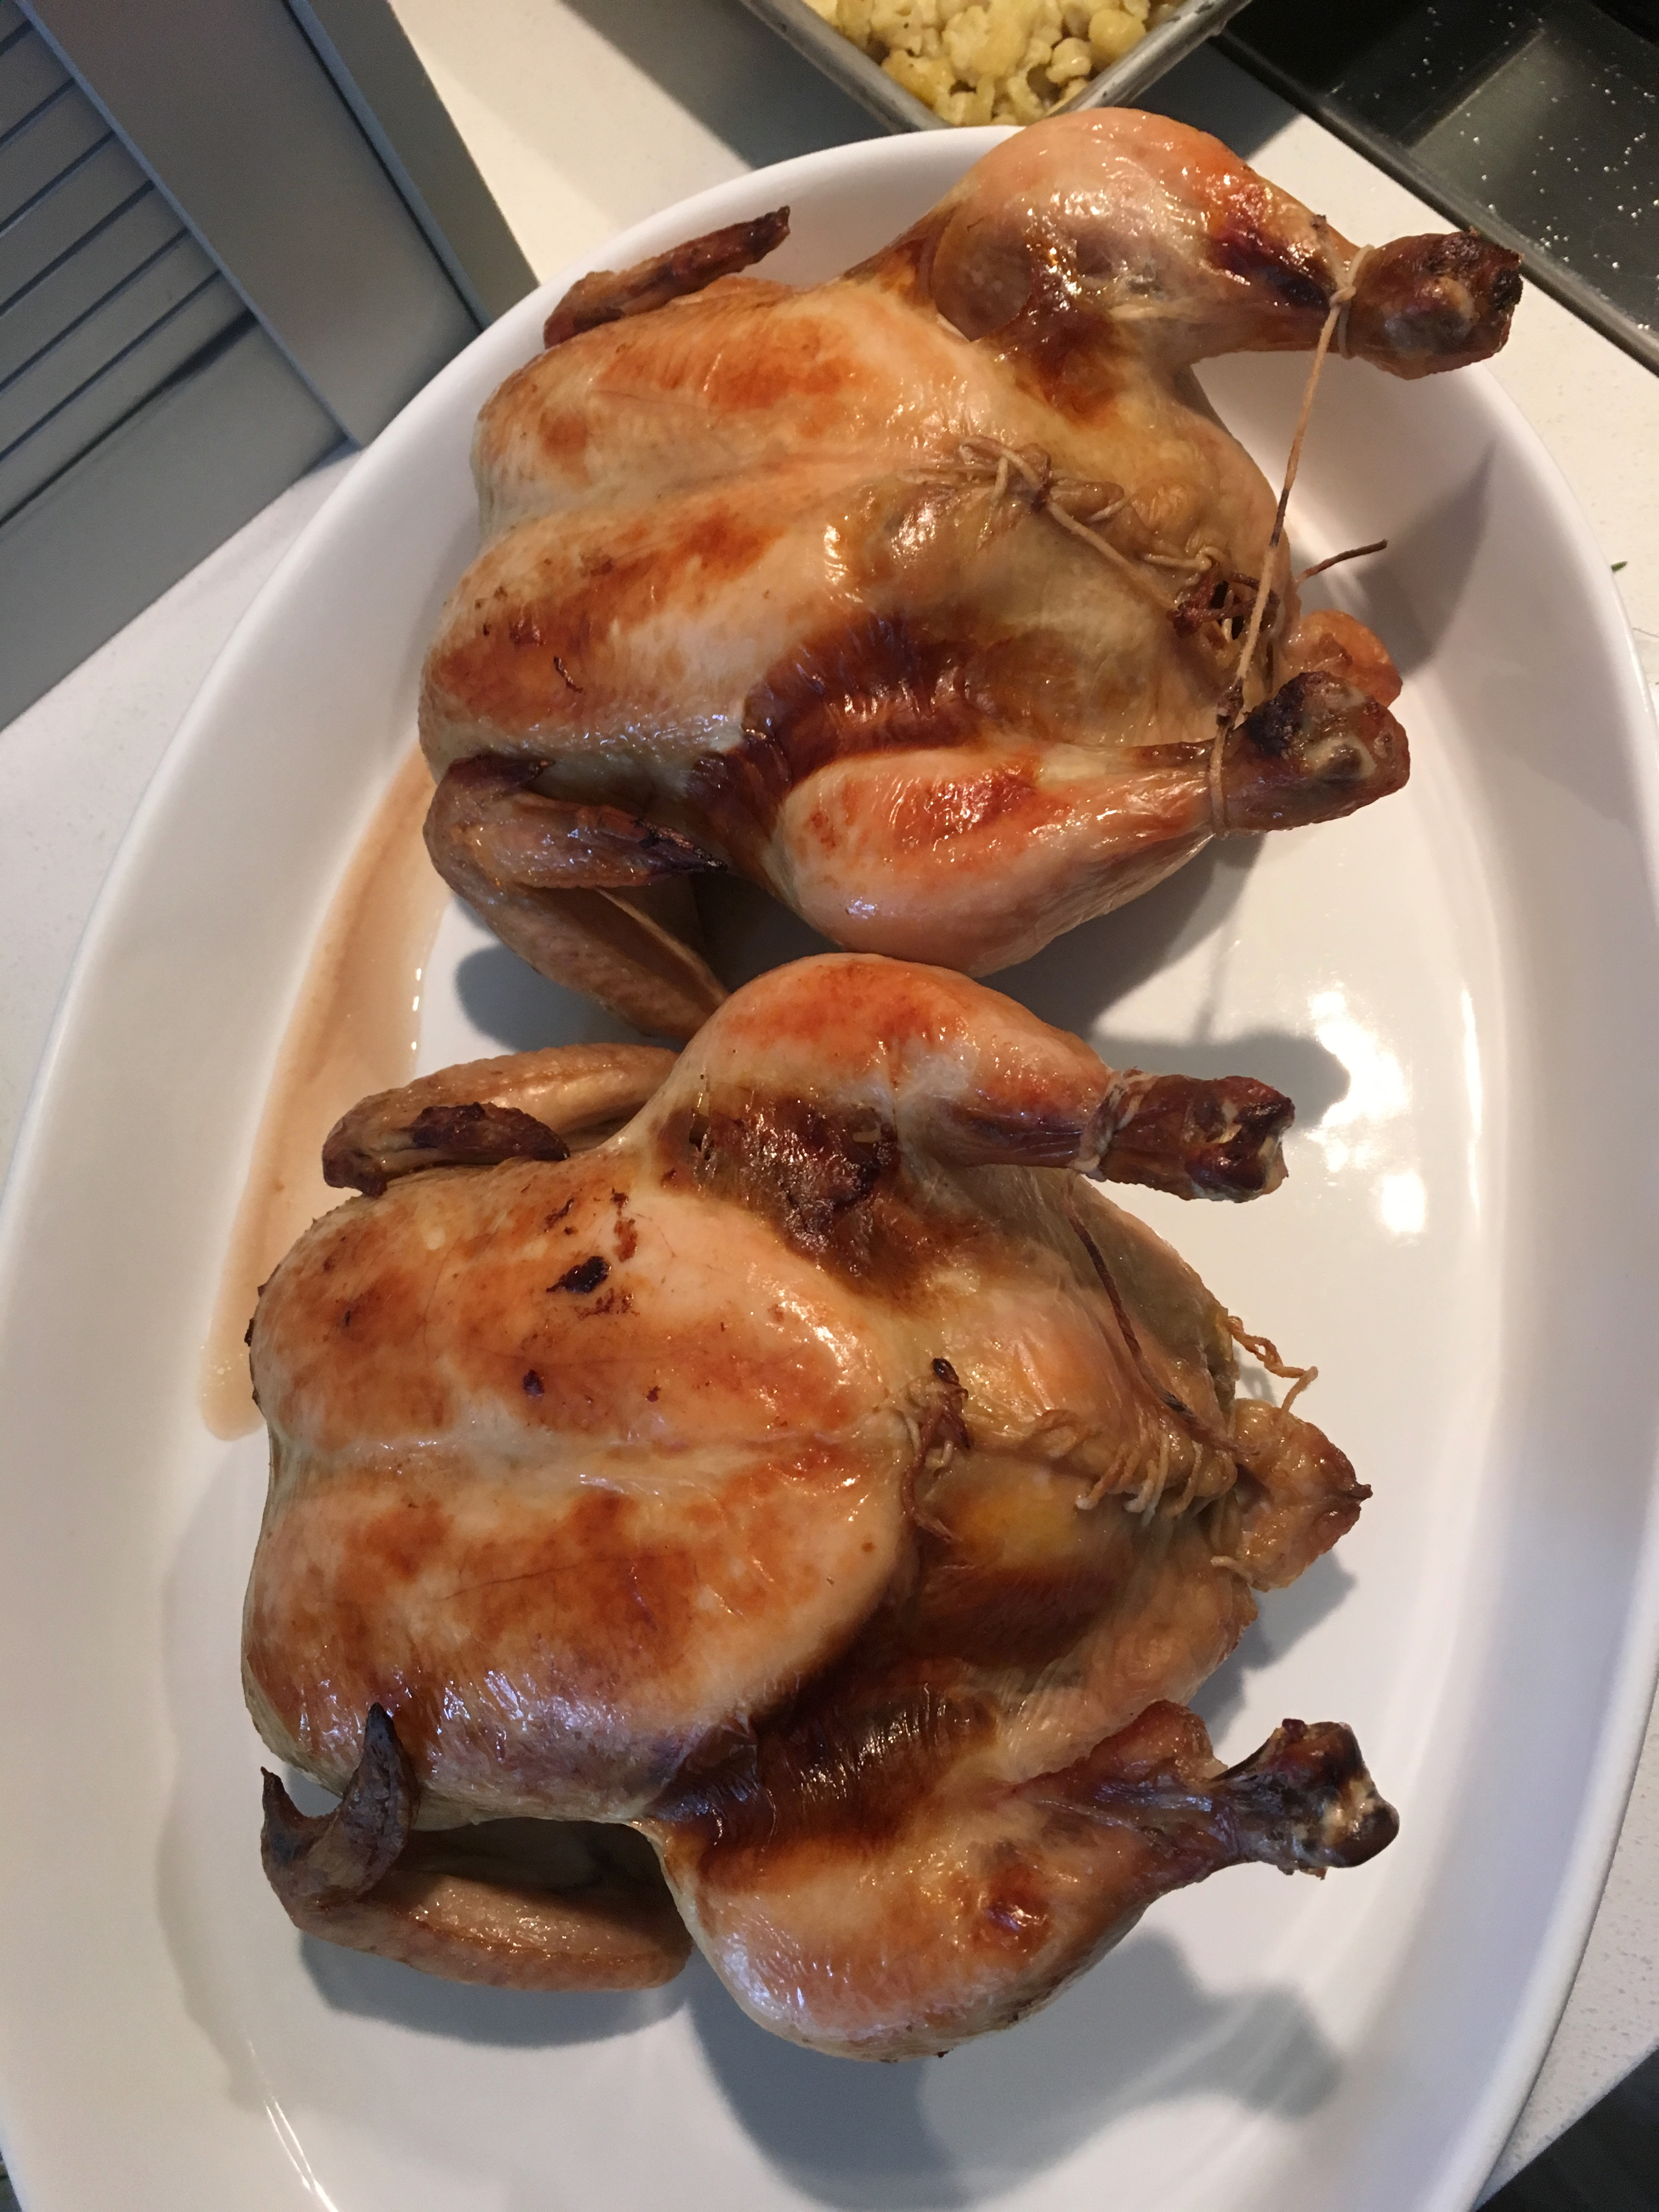
\includegraphics[width=0.25\textwidth]{\imageDir/\fileName/IMG_3228.jpg} \\
\end{tabular}
\end{table}

\end{document}



